\documentclass[11pt]{article}
\usepackage[utf8]{inputenc}
\usepackage{amsmath, amsfonts, amssymb}
\usepackage{graphicx}
\usepackage{geometry}
\usepackage{booktabs}
\usepackage{hyperref}
\usepackage{microtype}
\usepackage{xcolor}
\usepackage{tikz}
\usepackage[most]{tcolorbox}
\usepackage{placeins}

% Same notebox as homework3: third argument passes extra keys, which is how a breakable
% box sets coltext -- a plain \color inside one is lost at the page break.
\DeclareTColorBox{notebox}{ O{Note} O{blue} O{} }{
  breakable,
  colback=#2!5!white,
  colframe=#2!75!black,
  fonttitle=\bfseries,
  title={#1},
  #3
}

\geometry{margin=1in}

\title{Homework Assignment 1: Slab-Geometry Boltzmann Equation}
\author{Tal Ramot}
\date{\today}

\begin{document}

\maketitle

\section*{Introduction \& Case's Method}

The problem is the monoenergetic, steady-state Boltzmann equation in slab geometry, for an infinite homogeneous isotropic medium with an isotropic plane source at $x = 0$:
\begin{equation}
    \mu \frac{\partial \psi(x, \mu)}{\partial x} + \psi(x, \mu) = \frac{c}{2} \int_{-1}^1 \psi(x, \mu') d\mu' + \frac{1}{4\pi} \delta(x)
\end{equation}
with $c \in [0, 1)$ the scattering ratio and $\mu$ the direction cosine. Case (1953) looks for separable solutions $\psi_\nu(x,\mu) = e^{-x/\nu}\phi_\nu(\mu)$, which gives
\begin{equation}
    (\nu - \mu) \phi_\nu(\mu) = \frac{c\nu}{2} \int_{-1}^1 \phi_\nu(\mu') d\mu'
    \quad \xrightarrow{\ \int \phi_\nu d\mu = 1\ } \quad
    (\nu - \mu) \phi_\nu(\mu) = \frac{c\nu}{2}
\end{equation}
and splits into two spectra:
\begin{enumerate}
    \item \textbf{Discrete ($\nu \notin [-1,1]$).} Division by $\nu - \mu$ is legal, so $\phi_0^{\pm}(\mu) = c\nu_0 / [2(\nu_0 \mp \mu)]$, and normalization gives the characteristic equation
    \begin{equation}
        1 = c\nu_0 \operatorname{arctanh}(1/\nu_0)
    \end{equation}
    with exactly one pair of real roots $\pm\nu_0$, $\nu_0 > 1$, for $c \in (0,1)$.

    \item \textbf{Continuous ($\nu \in [-1,1]$).} Here $\nu - \mu$ vanishes at $\mu = \nu$, so the solution exists only as a distribution,
    \begin{equation}
        \phi_\nu(\mu) = \frac{c\nu}{2} \mathcal{P} \frac{1}{\nu - \mu} + \lambda(\nu)\delta(\mu - \nu),
        \qquad \lambda(\nu) = 1 - c\nu \operatorname{arctanh}(\nu)
    \end{equation}
    with $\mathcal{P}$ the Cauchy principal value and $\lambda$ fixed by the same normalization.
\end{enumerate}

The singular objects live in angle only. The scalar flux $\phi(x) = 2\pi\int_{-1}^1 \psi \,d\mu$ integrates them out, since $\int_{-1}^1 \phi_\nu(\mu)d\mu = 1$ by construction, leaving the ordinary integral
\begin{equation}
    \phi_{\text{tr}}(x) = \frac{1}{2} \int_0^1 \frac{e^{-|x|/\nu}}{N_\nu} d\nu,
    \qquad
    N_\nu = \nu \left[ \lambda^2(\nu) + \frac{\pi^2 c^2 \nu^2}{4} \right]
\end{equation}
whose integrand is smooth on $(0,1)$: it vanishes at $\nu \to 0$ through $e^{-|x|/\nu}$ and at $\nu \to 1$ through $\lambda \to -\infty$, so the quadrature is well behaved.

\section*{Question 1: Exact Scalar Flux Analysis}
\subsection*{Question 1a: Asymptotic and Transient Components}

The exact flux is the sum of the two contributions,
\begin{equation}
    \phi(x) = \phi_{\text{as}}(x) + \phi_{\text{tr}}(x),
    \qquad
    \phi_{\text{as}}(x) = \frac{e^{-|x|/\nu_0}}{2 N_0^+},
    \qquad
    N_0^+ = \frac{c}{2} \nu_0^3 \left[ \frac{c}{\nu_0^2 - 1} - \frac{1}{\nu_0^2} \right]
\end{equation}
$\nu_0$ is computed two ways: by bisection on $\operatorname{arctanh}(y)/y = 1/c$ with $y = 1/\nu_0 \in (0,1)$, and from the analytic fit
\begin{equation}
    \nu_0 \approx \frac{1}{\sqrt{1 - c^{p(c)}}},
    \qquad
    p(c) = 2.47412 + \frac{0.00363081}{c^2} - 0.0352458c + \frac{0.557498}{c}
\end{equation}
which agree to better than $5 \times 10^{-3}\,\%$ over $c = 0.5 \ldots 0.95$. All figures are produced with both.


\begin{figure}[hbt!]
    \centering
    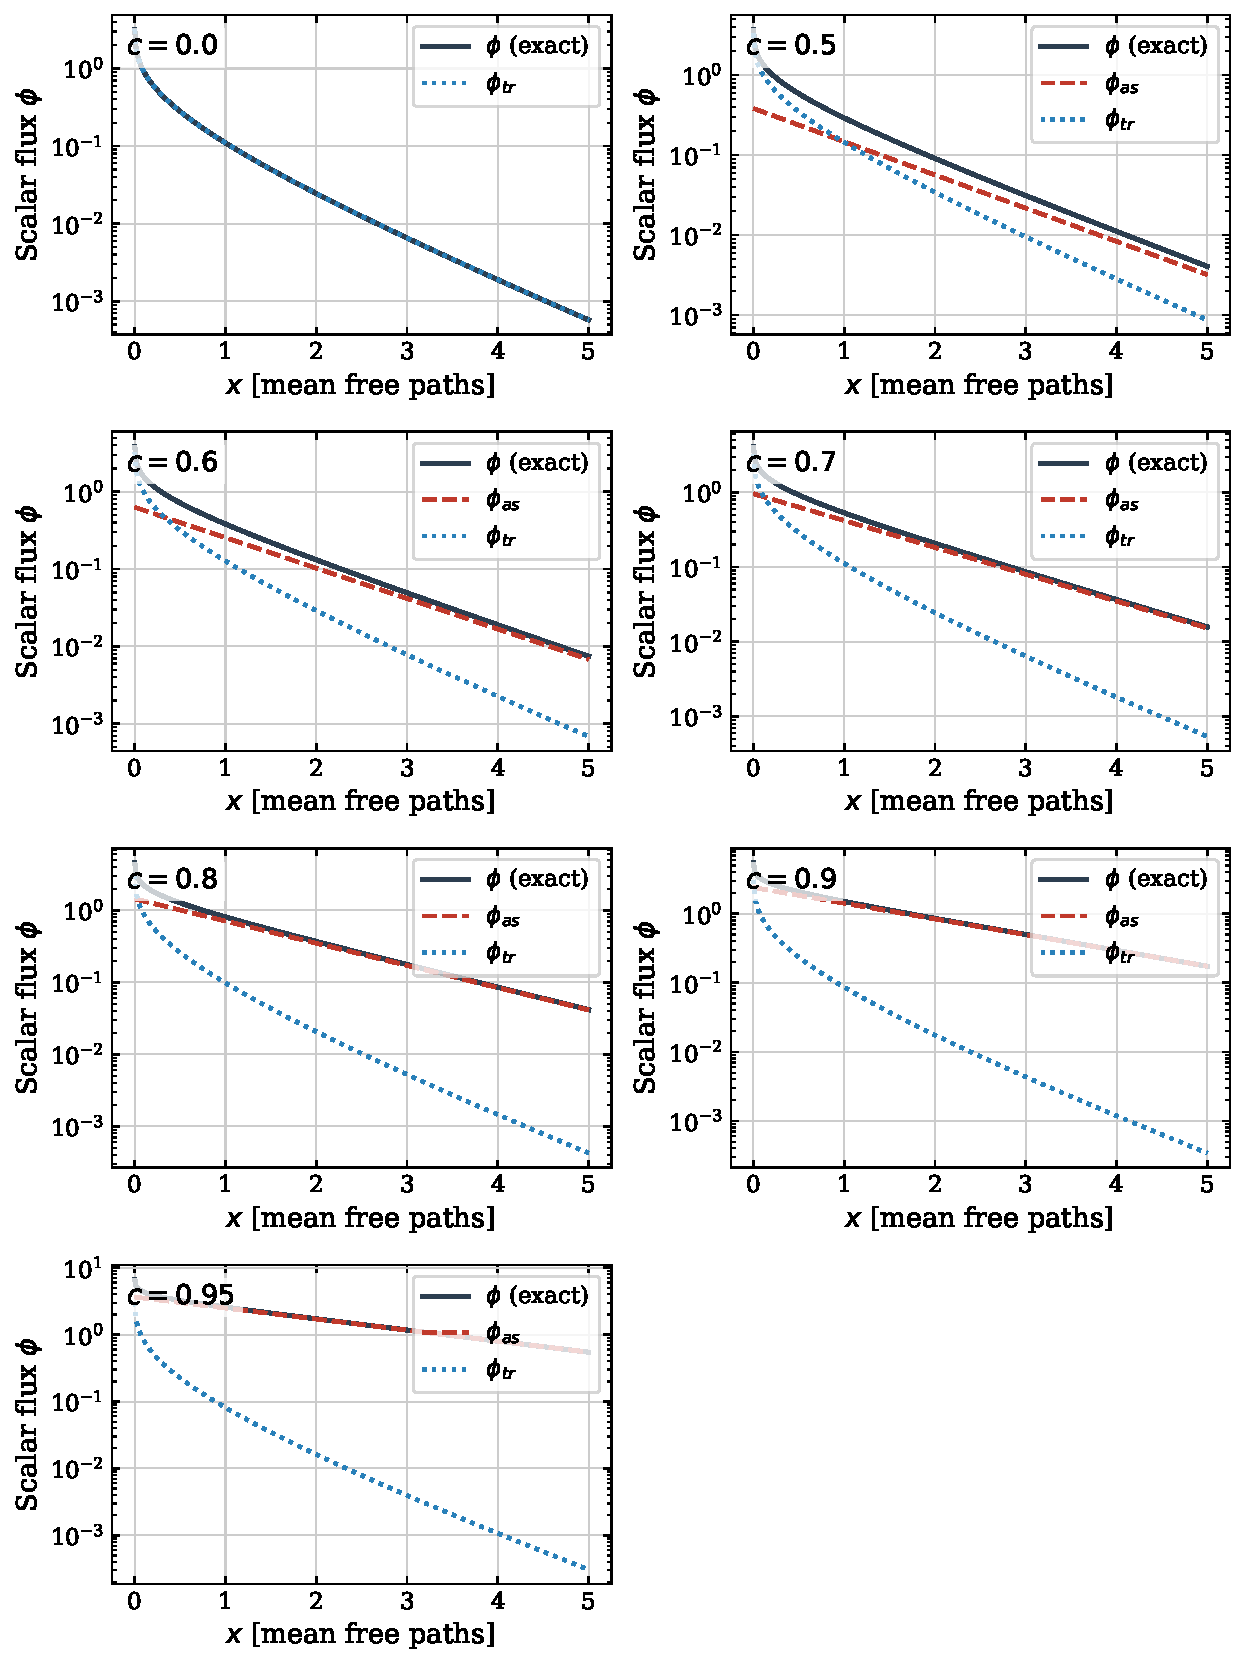
\includegraphics[width=0.85\textwidth]{figs/flux_components_numerical.pdf}
    \caption{The exact flux and its two components for each $c$. Note the log scale: the
    asymptotic part is a straight line, the transient part is not.}
    \label{fig:flux_components}
\end{figure}

\begin{figure}[hbt!]
    \centering
    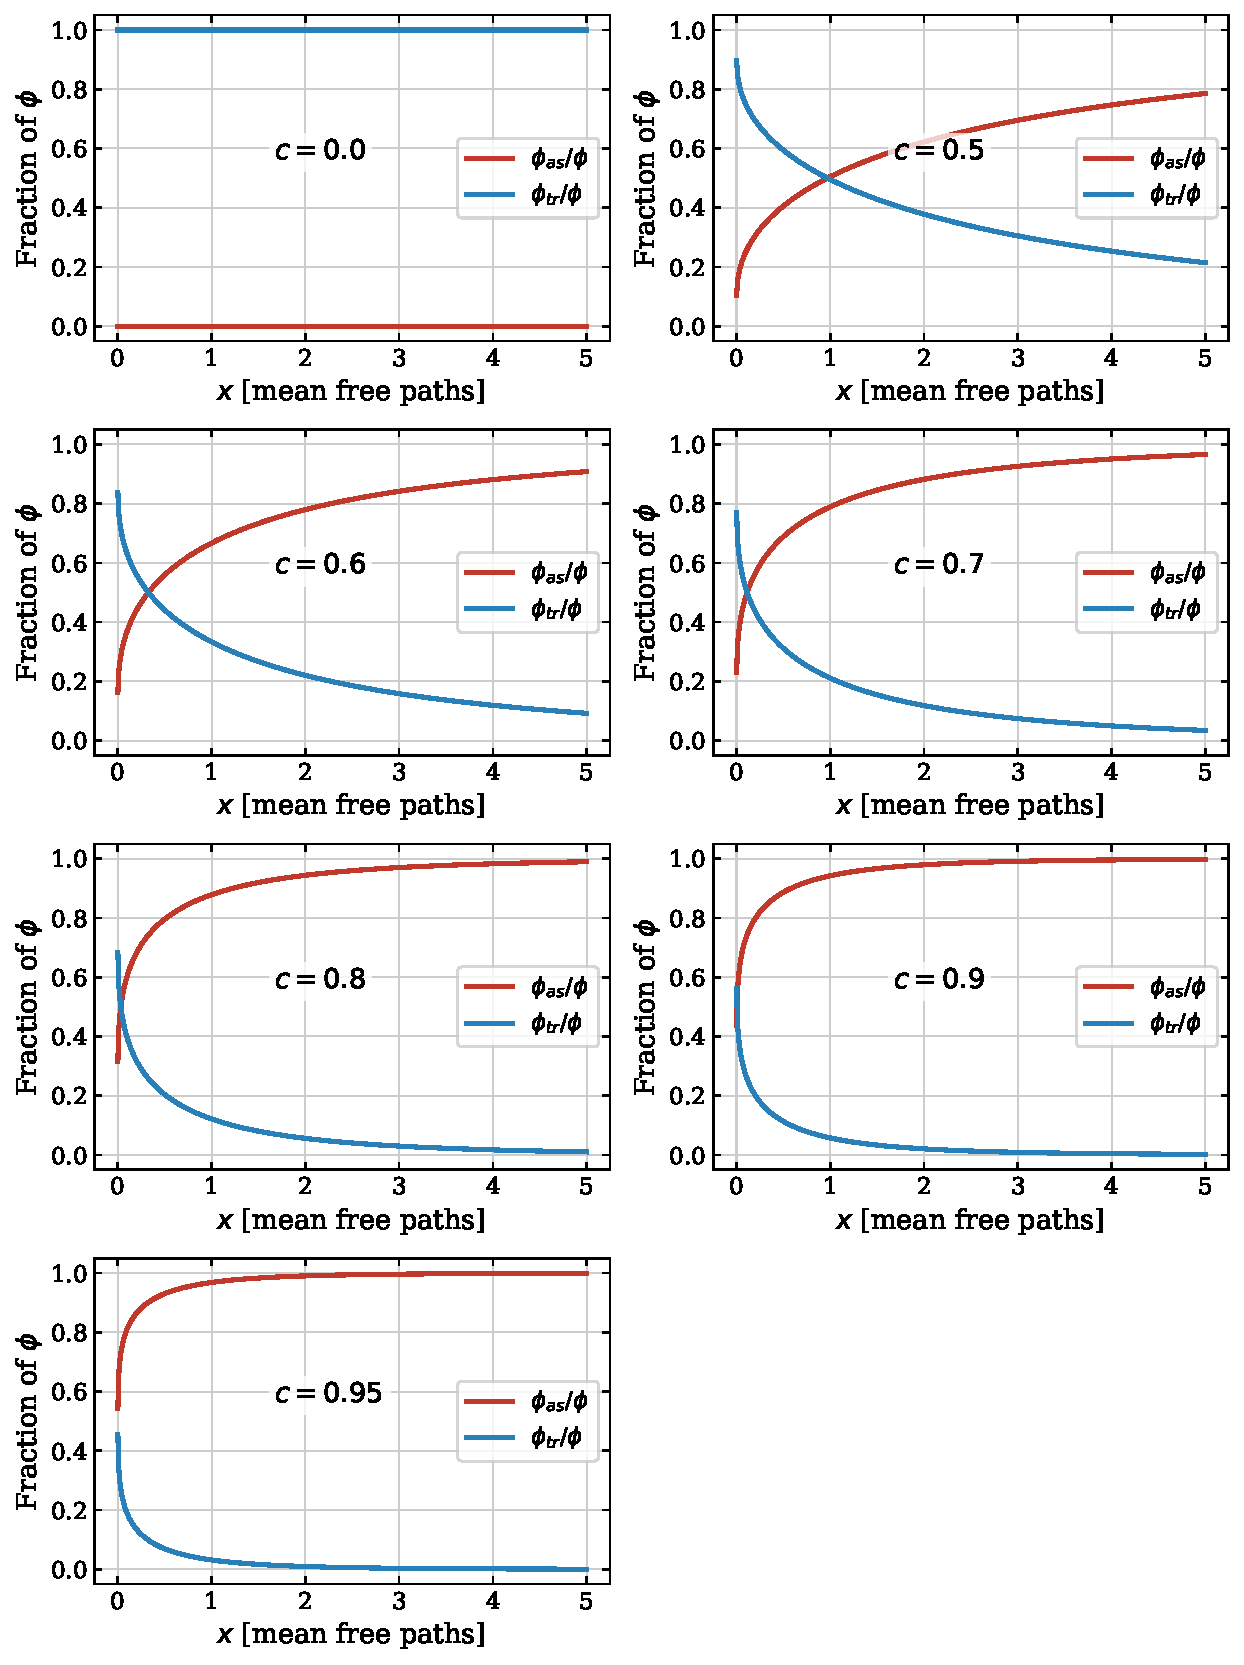
\includegraphics[width=0.85\textwidth]{figs/relative_contributions_numerical.pdf}
    \caption{The same two components as fractions of the total.}
    \label{fig:relative_contributions}
\end{figure}

\subsection*{Question 1b: Classical Diffusion Solution}

In mean free paths ($\Sigma_t = 1$) the diffusion equation for the same source is
\begin{equation}
    - D \phi''(x) + (1 - c) \phi(x) = \delta(x)
\end{equation}
and with the $P_1$ value $D = 1/3$ its Green's function is
\begin{equation}
    \phi_{\text{class}}(x) = \frac{\sqrt{3}}{2\sqrt{1-c}} e^{-\sqrt{3(1-c)} |x|}
\end{equation}

\subsection*{Question 1c: Asymptotic Diffusion Solution}

Matching the diffusion length to the exact eigenvalue, $L = \nu_0$, fixes $D_{\text{as}} = (1-c)\nu_0^2$ and gives
\begin{equation}
    \phi_{\text{as,diff}}(x) = \frac{1}{2(1-c)\nu_0} e^{-|x|/\nu_0}
\end{equation}
which is exactly Case's asymptotic mode: this approximation reproduces $\phi_{\text{as}}$ by construction and errs only by the transient part.

\subsection*{Question 1d: Relative Error of Diffusion Approximations}

\begin{equation}
    \text{Relative Error (\%)} = \frac{|\phi_{\text{approx}}(x) - \phi_{\text{exact}}(x)|}{\phi_{\text{exact}}(x)} \times 100\%
\end{equation}

\begin{figure}[hbt!]
    \centering
    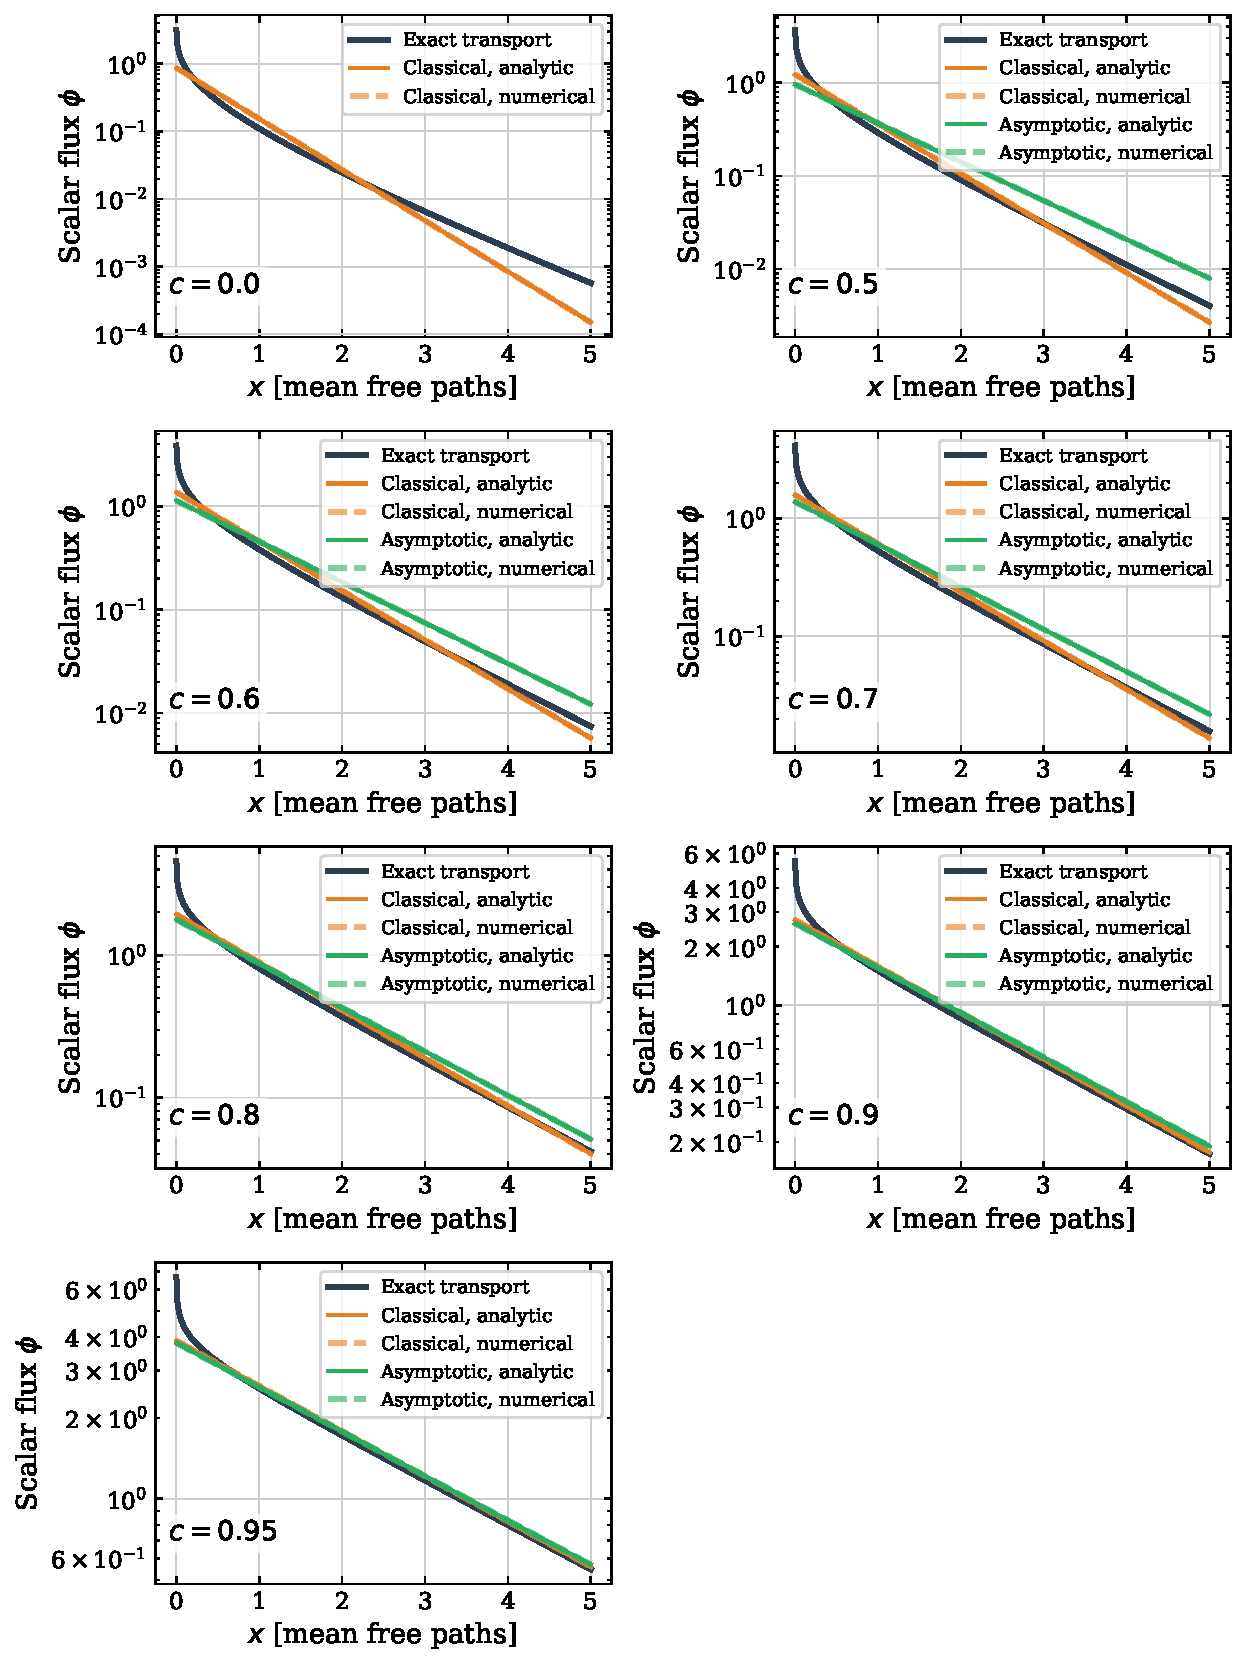
\includegraphics[width=0.85\textwidth]{figs/diffusion_comparison_numerical.pdf}
    \caption{Exact scalar flux against the classical and asymptotic diffusion approximations, for $c = 0, 0.5, 0.6, 0.7, 0.8, 0.9, 0.95$. Each approximation appears both as its closed form and as the numerical solution of Question 2. The two agree to $2 \times 10^{-8}\,\%$ and are indistinguishable here.}
    \label{fig:diffusion_comparison}
\end{figure}

\begin{figure}[hbt!]
    \centering
    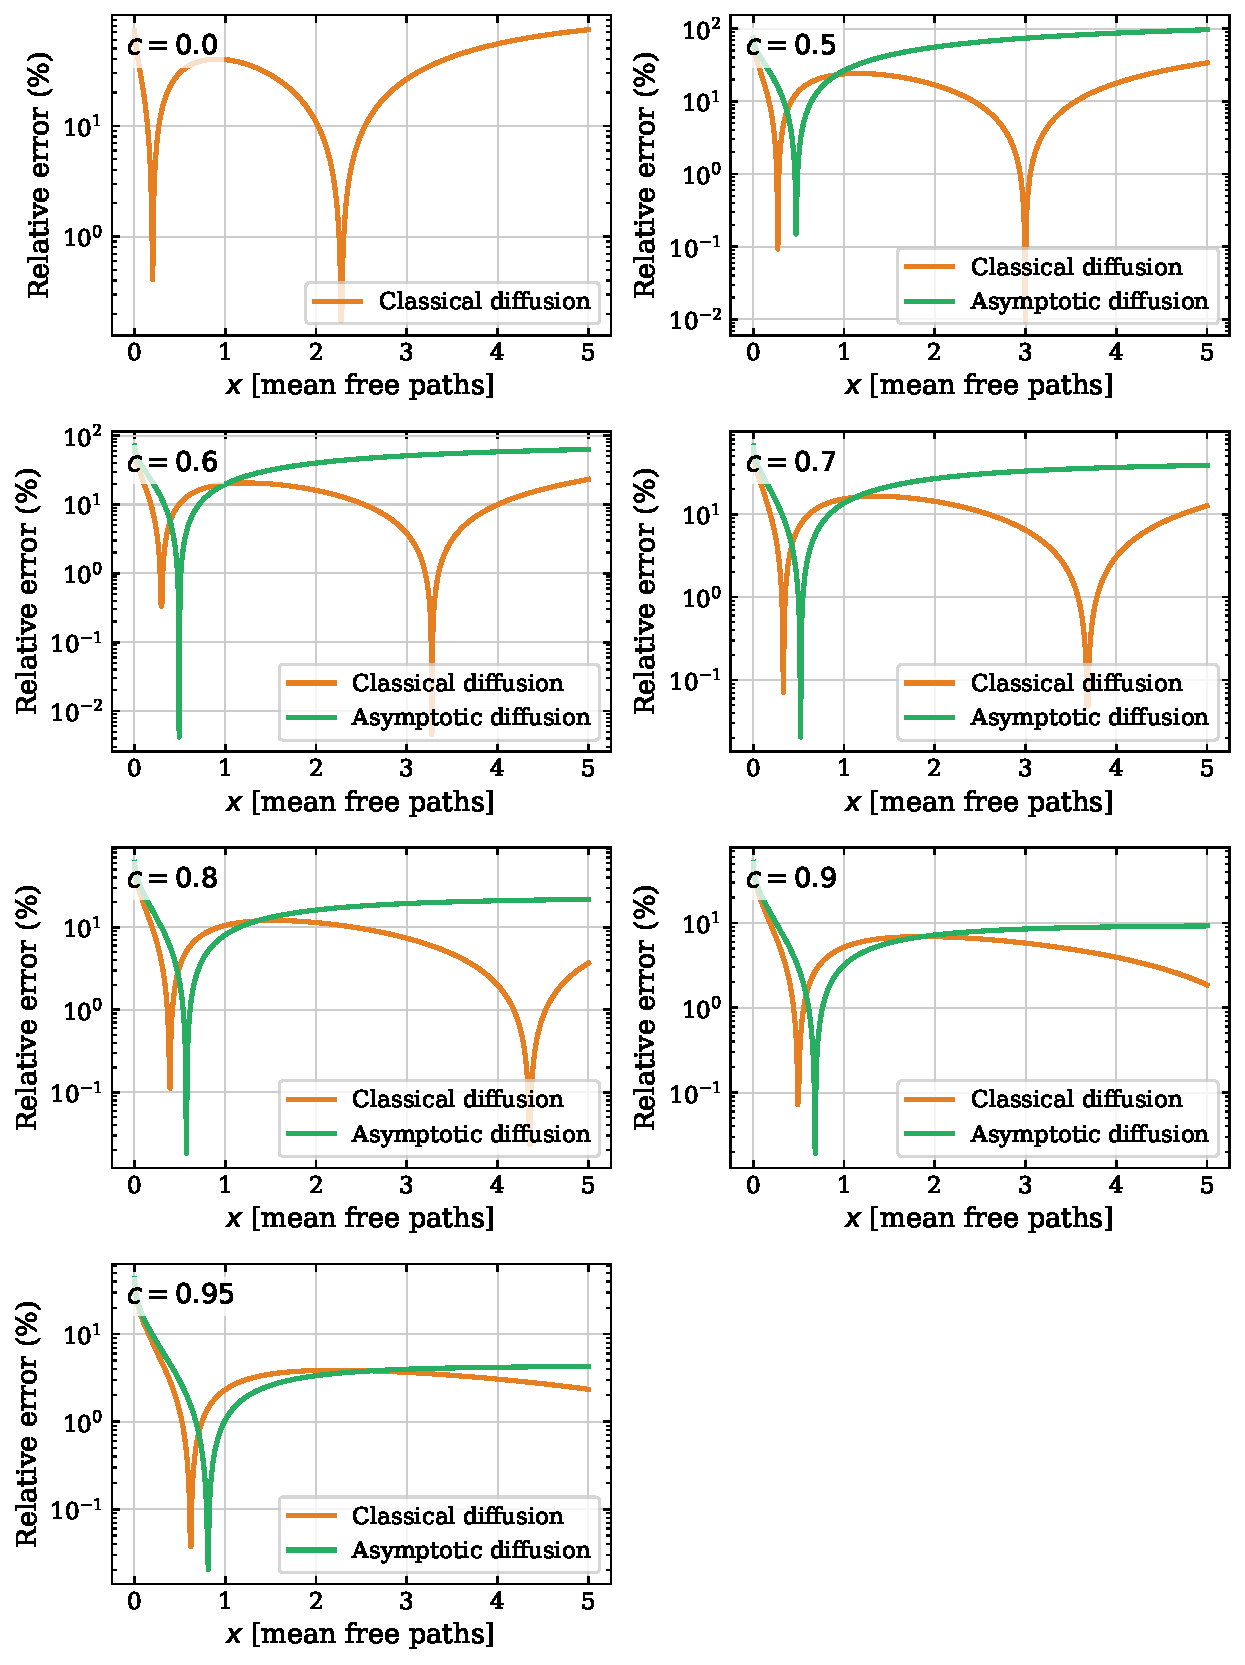
\includegraphics[width=0.85\textwidth]{figs/diffusion_errors_numerical.pdf}
    \caption{Relative error of each diffusion approximation against the \emph{exact transport} solution, which is the modelling error asked for in 1d.}
    \label{fig:diffusion_errors}
\end{figure}

\newpage 
\section*{Question 2: Numerical Code for the Diffusion Equation}

The medium is symmetric, so the problem is solved on the half-domain $x \in [0,a]$, where it is source-free:
\begin{equation}
    - D \phi''(x) + (1 - c) \phi(x) = 0
    \quad\Longrightarrow\quad
    \frac{d}{dx} \begin{pmatrix} y_1 \\ y_2 \end{pmatrix} = \begin{pmatrix} y_2 \\ \frac{1-c}{D} y_1 \end{pmatrix},
    \qquad y_1 = \phi,\; y_2 = \phi'
\end{equation}

\paragraph{The delta source.} We are \textit{transforming} the source into a BC at $x=0$. Integrating across the origin gives $-D[\phi'(0^+) - \phi'(0^-)] = 1$, and evenness of the infinite-medium solution gives half the source streaming every way (which makes a lot of physical sense):
\begin{equation}
    \phi'(0^+) = -\frac{1}{2D},
    \qquad \iff \qquad
    J(0^+) = -D\phi'(0^+) = \frac{1}{2}
\end{equation}

\paragraph{The outer boundary.} $x = a$ is a truncation, not a surface. Zero flux there (something we had tried) would force a $100\,\%$ error at $x = a$ ,so instead we use the condition
\begin{equation}
    \phi'(a) = -\kappa \phi(a) \qquad \text{for} \qquad \kappa = \sqrt{\Sigma_a / D}
\end{equation}
which is satisfied by $e^{-\kappa x}$. Thus the truncation is exact for any $a$. We take $a = 10/\kappa$ in the presented plots.

\paragraph{One integration.} The equation is linear and homogeneous away from the source, so the solution is proportional to its starting amplitude and no root-finding is needed. We integrate once from $a$ to $0$ - the direction in which the solution grows, which is the stable one - from $[y_1, y_2]^T = [1, -\kappa]^T$, then rescale by $[-1/(2D)]/y_2(0)$ to enforce the source condition. Both classic \& asymptotic approximations use this one solver, since
\begin{equation}
    \Sigma_a = 1 - c, \qquad D_{\text{classical}} = \frac{1}{3}, \qquad D_{\text{asymptotic}} = (1-c)\,\nu_0^2
\end{equation}

\paragraph{Verification.} The solver reproduces the closed form to $2 \times 10^{-8}\,\%$ for both approximations at $c = 0.5, 0.7, 0.9$. Figures~\ref{fig:diffusion_comparison}--\ref{fig:q2_error_profiles} show the numerical solution against the analytic Green's function, the relative error across the domain, and the convergence of the shooting solver with tolerance.

\begin{figure}[hbt!]
    \centering
    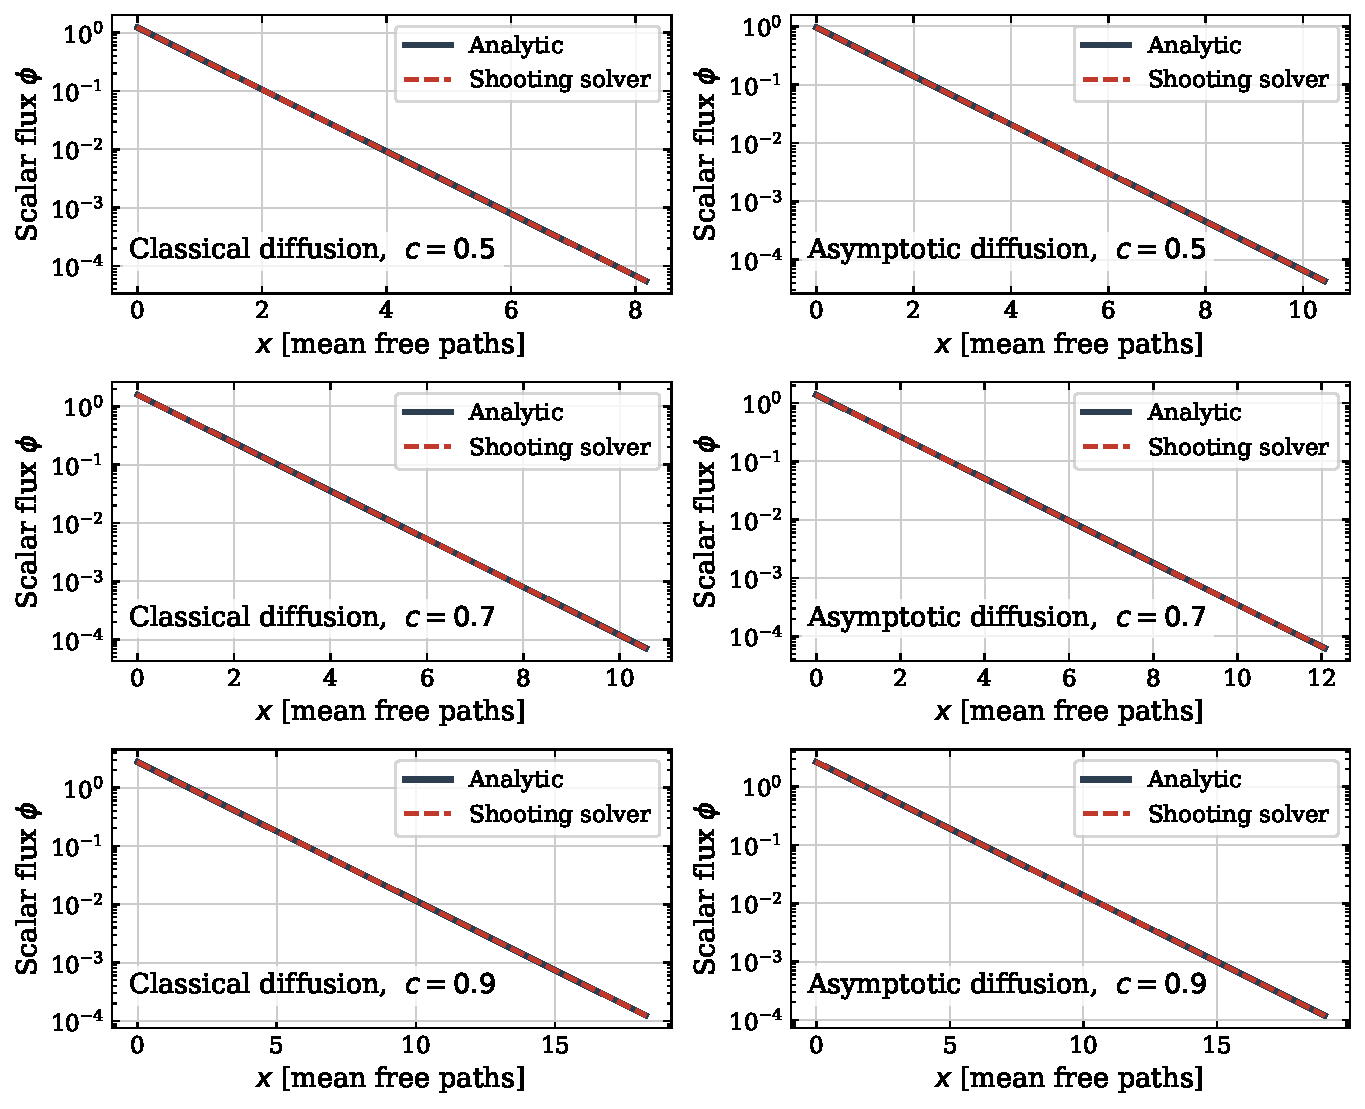
\includegraphics[width=0.9\textwidth]{figs/q2_solution_comparison.pdf}
    \caption{Numerical solution against the analytic diffusion Green's function, both approximations at $c = 0.5, 0.7, 0.9$.}
    \label{fig:q2_solution_comparison}
\end{figure}

\begin{figure}[hbt!]
    \centering
    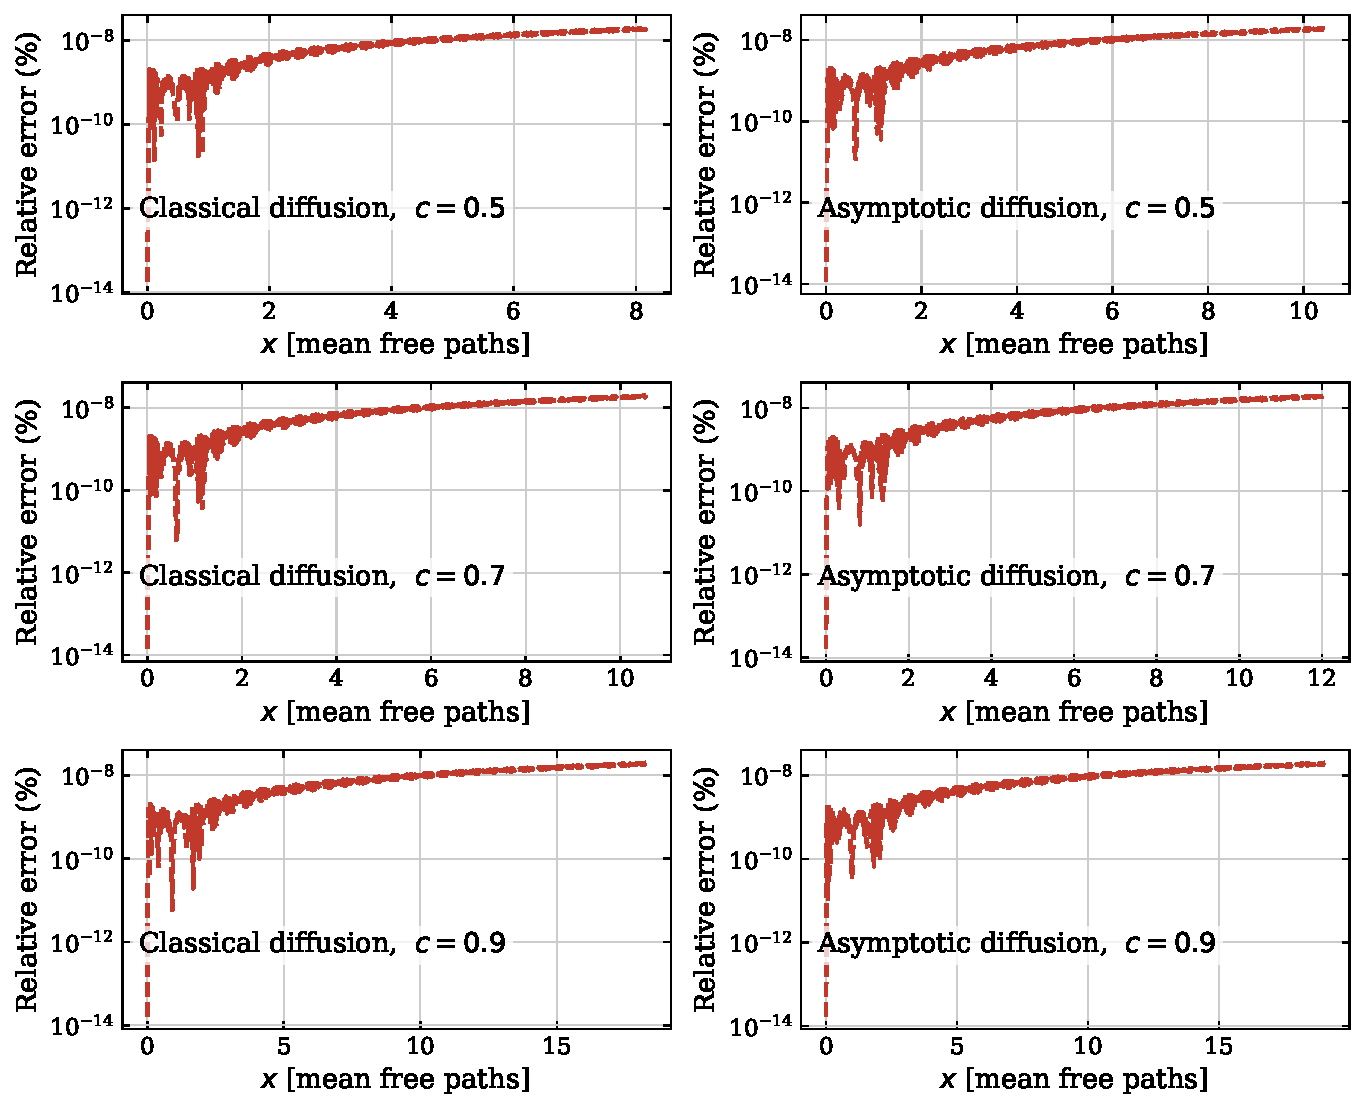
\includegraphics[width=0.9\textwidth]{figs/q2_error_profiles.pdf}
    \caption{Relative error across the domain. With the radiation condition it stays flat instead of diverging at the outer edge.}
    \label{fig:q2_error_profiles}
\end{figure}

\begin{figure}[hbt!]
    \centering
    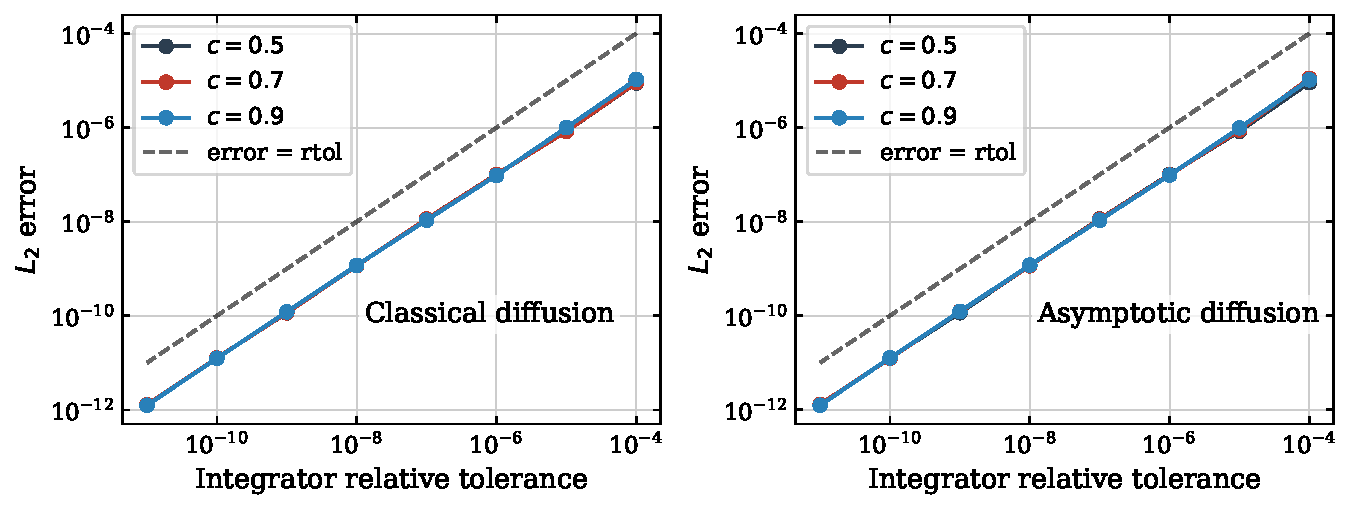
\includegraphics[width=0.9\textwidth]{figs/q2_convergence.pdf}
    \caption{Tolerance convergence of the shooting solver.}
    \label{fig:q2_convergence}
\end{figure}

\newpage
\section*{Question 3: Critical Half-Thickness and Critical Radius}

\subsection*{The Eigenvalue for $c > 1$}
The discrete eigenvalue leaves the real axis. With $\nu_0 = i|\nu_0|$, $k_0 = 1/|\nu_0|$ and $\operatorname{arctanh}(ik) = i\arctan(k)$, the characteristic equation becomes real again,
\begin{equation}
    c \arctan(k_0) = k_0
\end{equation}
the form tabulated by Case, de Hoffmann \& Placzek (Table 8, Part II), which the root reproduces to $5 \times 10^{-6}$. The fit of Question 1 continues onto this branch by itself, its radicand simply changing sign:
\begin{equation}
    |\nu_0(c)| = \frac{1}{\sqrt{c^{p(c)} - 1}}
\end{equation}
accurate to $10^{-4}\,\%$ at $c = 1.02$ and $0.10\,\%$ at $c = 2$. An imaginary $\nu_0$ makes the asymptotic flux trigonometric, which is what allows a finite critical system:
\begin{equation}
    \phi_{\text{as}}(x) = A \cos\!\left(\frac{\Sigma_t x}{|\nu_0|}\right), \qquad
    \phi_{\text{as}}(r) = A \frac{\sin\!\left(\Sigma_t r / |\nu_0|\right)}{\Sigma_t r}
\end{equation}
the sine being excluded in the slab by symmetry, the cosine in the sphere by regularity.

\subsection*{The Criticality Relations}
The asymptotic flux extrapolates to zero a distance $z_0(c)$ outside the surface. Placing the quarter-wave zero of the cosine and the first zero of the sine there gives, in mean free paths,
\begin{equation}
    \frac{a}{2} = \frac{\pi}{2}\,|\nu_0(c)| - z_0(c), \qquad
    \Sigma_t R_c = \pi\,|\nu_0(c)| - z_0(c)
    \label{eq:q3relations}
\end{equation}
No diffusion coefficient enters, so these are exact transport in that sense. They are still asymptotic, in that the transient flux near the surface is neglected (and the sphere uses the plane Milne $z_0$, without the Winslow curvature correction). The extrapolation distance comes from the expansion about $c = 1$,
\begin{equation}
    z_0(c) = 0.710446 \left[ \frac{1}{c} + q\,\frac{(1-c)^2}{c} + \mathcal{O}\!\left(\frac{(1-c)^3}{c}\right) \right]
    \label{eq:z0fit}
\end{equation}
whose leading term is exact in the sense that $0.710446/c = 0.710446\,\nu_0\operatorname{arctanh}(1/\nu_0)$, with $0.710446$ Hopf's constant.

\begin{notebox}[The sign of the quadratic correction in \eqref{eq:z0fit}]
The notes print $q = -0.0199$. Case's Table 23 has $c\,z_0(c)$ rising away from $0.710446$ on
\emph{both} sides of $c = 1$, which a negative $q$ cannot reproduce, while $q = +0.0199$ matches
the table to its four printed digits at $c = 0.9$ and $c = 1.1$ - so the minus sign looks like
a transcription error. It matters little here: over $1.02 < c < 2$ the two signs differ by at
most $3.2\,\%$ in $a/2$, and by under $0.07\,\%$ below $c = 1.2$. Results are quoted with the
printed sign.
\end{notebox}

\subsection*{Results}
\begin{table}[hbt!]
    \centering
    \begin{tabular}{lrrrrr}
        \toprule
        $c$ & $|\nu_0(c)|$ & $z_0(c)$ & $a/2$ & $\Sigma_t R_c$ & error in $a/2$ \\
        \midrule
        1.02 & 4.050190 & 0.696510 & 5.665513 & 12.027537 & $0.0001\,\%$ \\
        1.05 & 2.531781 & 0.676582 & 3.300331 & 7.277244 & $0.0025\,\%$ \\
        1.10 & 1.756653 & 0.645731 & 2.113612 & 4.872955 & $0.0128\,\%$ \\
        1.20 & 1.198272 & 0.591567 & 1.290674 & 3.172916 & $0.0667\,\%$ \\
        1.30 & 0.946021 & 0.545518 & 0.940488 & 2.426495 & $0.1777\,\%$ \\
        1.40 & 0.793813 & 0.505846 & 0.741072 & 1.987990 & $0.3592\,\%$ \\
        1.50 & 0.689210 & 0.471274 & 0.611333 & 1.693941 & $0.6116\,\%$ \\
        1.60 & 0.611746 & 0.440848 & 0.520080 & 1.481008 & $0.9535\,\%$ \\
        1.70 & 0.551520 & 0.413834 & 0.452491 & 1.318817 & $1.3672\,\%$ \\
        1.80 & 0.503065 & 0.389665 & 0.400547 & 1.190759 & $1.8831\,\%$ \\
        1.90 & 0.463074 & 0.367892 & 0.359503 & 1.086897 & $2.4781\,\%$ \\
        2.00 & 0.429411 & 0.348154 & 0.326364 & 1.000881 & $3.1859\,\%$ \\
        \bottomrule
    \end{tabular}
    \caption{Critical dimensions in mean free paths, from the approximate $|\nu_0(c)|$ and the printed $z_0$ fit ($q = -0.0199$). The last column is the departure of $a/2$ from a reference using the transcendental root and Case's Table 23.}
    \label{tab:q3}
\end{table}

Both dimensions fall steeply with $c$ - a barely multiplying system must be many mean free
paths across, because $|\nu_0| \to \infty$ as $c \to 1^+$.

\begin{notebox}[How good is the two-term fit for $z_0$?]
Table~\ref{tab:q3} uses the fitted $|\nu_0|$ and $z_0$ of \eqref{eq:z0fit} rather than the
transcendental root and Case's table, and the error that costs is almost all $z_0$: the
eigenvalue fit stays under $0.11\,\%$, while the two-term $z_0$ expansion reaches $2.6\,\%$ by
$c = 2$, where $(1-c)^3$ is no smaller than $(1-c)^2$. Because $z_0$ is subtracted while
$|\nu_0|$ is multiplied by $\pi$ or $\pi/2$, the same absolute error in $z_0$ hurts $a/2$ about
twice as much as $R_c$. The total stays under $0.1\,\%$ to $c \approx 1.25$ and reaches a few
per cent by $c = 2$ (Figure~\ref{fig:q3_critical}). Everything after this table uses the exact
inputs instead.
\end{notebox}

\begin{figure}[hbt!]
    \centering
    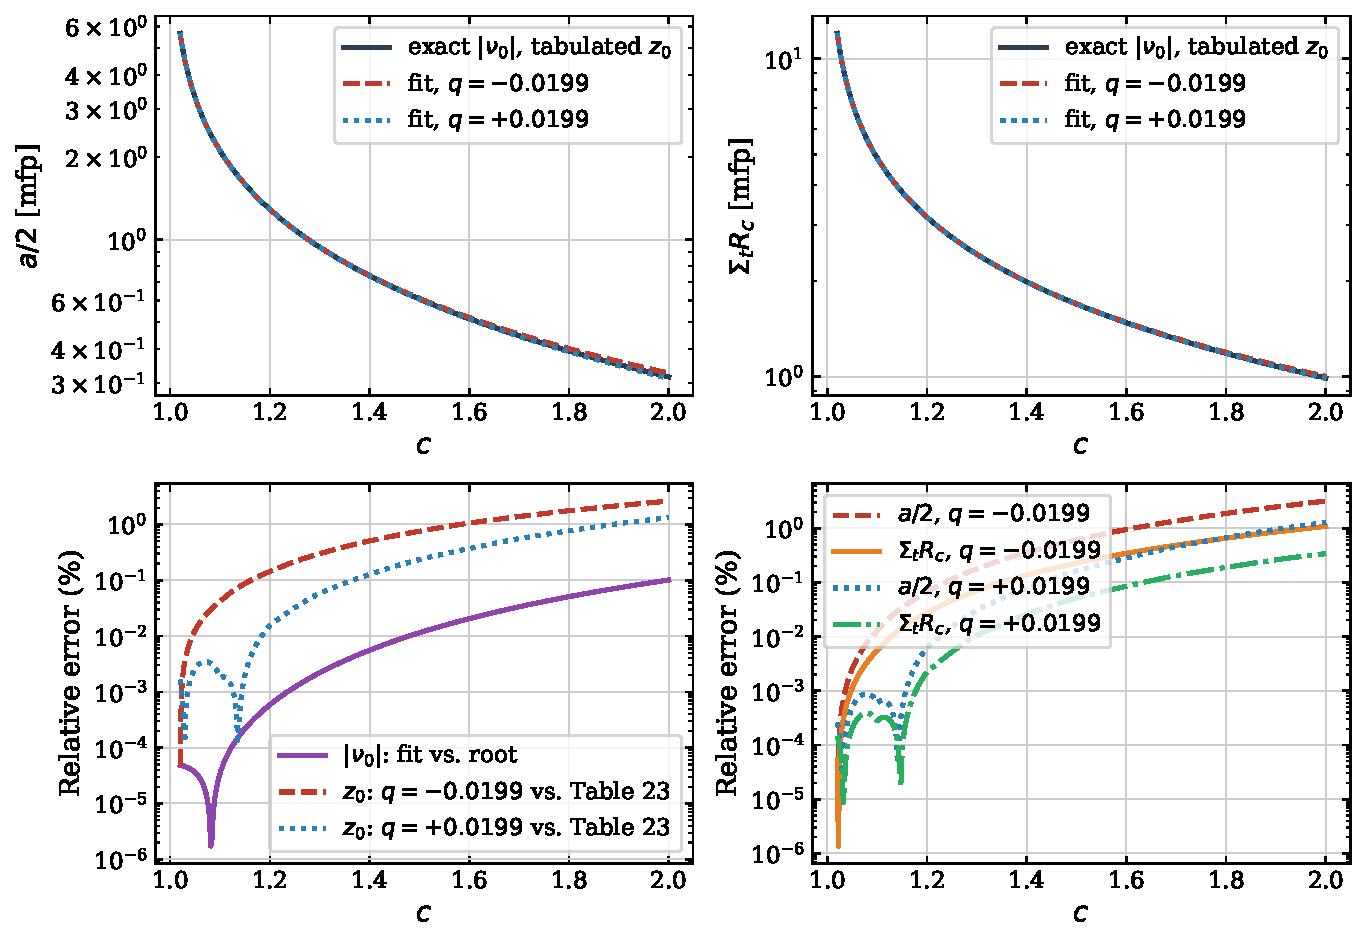
\includegraphics[width=\textwidth]{figs/q3_critical_dimensions.pdf}
    \caption{Critical half-thickness and radius for $1.02 < c < 2$ (top), and the errors of the approximate inputs and of the resulting dimensions (bottom).}
    \label{fig:q3_critical}
\end{figure}


\subsection*{Parts 3(b) and 3(c): Marshak and Mark Conditions}
A multiplying medium has $\Sigma_a = 1 - c < 0$, so classical diffusion gives a Helmholtz equation
\begin{equation}
    -D \nabla^2 \phi + (1-c)\phi = 0
    \quad\Longrightarrow\quad
    \nabla^2 \phi + B^2 \phi = 0, \qquad B^2 = \frac{c-1}{D} = 3(c-1)
\end{equation}
whose solutions are the \emph{same} shapes $\cos(Bx)$ and $\sin(Br)/r$. Diffusion therefore leaves \eqref{eq:q3relations} unchanged in form and only replaces the two inputs:
\begin{equation}
    |\nu_0(c)| \;\longrightarrow\; \frac{1}{B} = \frac{1}{\sqrt{3(c-1)}},
    \qquad
    z_0(c) \;\longrightarrow\;
    \begin{cases}
        2/3 & \text{Marshak} \\[2pt]
        1/\sqrt{3} & \text{Mark}
    \end{cases}
\end{equation}
Marshak sets the incoming partial current to zero, $\phi/4 + D\phi'/2 = 0$, so $z_0 = \ell_0 = 2D = 2/3$. Mark sets the incoming angular flux to zero along $\mu = 1/\sqrt{3}$, so $z_0 = \ell_0 = \sqrt{3}D \approx 0.5774$. Neither input carries the true $c$-dependence: $1/B$ is only the $c \to 1^+$ limit of $|\nu_0|$, and both $z_0$ are constants while the transport $z_0(c) \approx 0.7104/c$ halves across the range.

\begin{table}[hbt!]
    \centering
    \begin{tabular}{lrrrrrr}
        \toprule
        & \multicolumn{3}{c}{$a/2$} & \multicolumn{3}{c}{$\Sigma_t R_c$} \\
        \cmidrule(lr){2-4}\cmidrule(lr){5-7}
        $c$ & transport (a) & Marshak (b) & Mark (c) & transport (a) & Marshak (b) & Mark (c) \\
        \midrule
        1.02 & 5.665513 & 5.746082 & 5.835399 & 12.027537 & 12.158832 & 12.248148 \\
        1.05 & 3.300331 & 3.389112 & 3.478428 & 7.277244 & 7.444891 & 7.534207 \\
        1.10 & 2.113612 & 2.201202 & 2.290518 & 4.872955 & 5.069071 & 5.158387 \\
        1.20 & 1.290674 & 1.361223 & 1.450539 & 3.172916 & 3.389112 & 3.478428 \\
        1.30 & 0.940488 & 0.989098 & 1.078414 & 2.426495 & 2.644863 & 2.734179 \\
        1.40 & 0.741072 & 0.767268 & 0.856584 & 1.987990 & 2.201202 & 2.290518 \\
        1.50 & 0.611333 & 0.615883 & 0.705200 & 1.693941 & 1.898433 & 1.987749 \\
        1.60 & 0.520080 & 0.504136 & 0.593452 & 1.481008 & 1.674938 & 1.764255 \\
        1.70 & 0.452491 & 0.417286 & 0.506602 & 1.318817 & 1.501238 & 1.590555 \\
        1.80 & 0.400547 & 0.347278 & 0.436594 & 1.190759 & 1.361223 & 1.450539 \\
        1.90 & 0.359503 & 0.289290 & 0.378606 & 1.086897 & 1.245246 & 1.334562 \\
        2.00 & 0.326364 & 0.240233 & 0.329549 & 1.000881 & 1.147133 & 1.236449 \\
        \bottomrule
    \end{tabular}
    \caption{Critical dimensions in mean free paths from the three treatments: exact transport (3a), Marshak diffusion (3b) and Mark diffusion (3c).}
    \label{tab:q3bc}
\end{table}

\subsection*{Parts 3(d) and 3(e): Asymptotic Diffusion}
Every part of this question uses the same relations \eqref{eq:q3relations}, so a part is fixed
by naming \emph{two} inputs, not one: the relaxation length $\ell$ inside $\cos(x/\ell)$ (which is where the $\nu_0(c)$ term comes from), and
the boundary closure. Parts (b) and (c) take $\ell = 1/\sqrt{3(c-1)}$ which is actually the approximation of $\nu_0(c)$ in the diffusive $c\to 1$ limit. Parts (a), (d) and (e)
take $\ell = |\nu_0|$. \textbf{Once the theory fixes $\ell$, \textit{the closure} (e.g. $z_0$, but soon we'll notice that it's case-dependent) is the only freedom left.}

\paragraph{The closure has two encodings.} A boundary condition delivers the ratio
$\ell_0 = \phi/|\phi'|$ at the surface, but \eqref{eq:q3relations} uses $z_0$, the point where the cosine itself vanishes. For $\phi = \cos(x/\ell)$ those are not the same number:
\begin{equation}
    \ell_0 = \nu_0 \tan\!\left(\frac{z_0}{\nu_0}\right),
    \qquad\qquad
    z_0 = \nu_0 \arctan\!\left(\frac{\ell_0}{\nu_0}\right)
    \label{eq:l0z0}
\end{equation}
They agree only when $\ell_0 \ll \nu_0$, which is the $c \to 1^+$ limit where $\nu_0$ diverges.
Writing $z_0 = \ell_0 = 2D$, as parts (b) and (c) do above, is therefore that limit taken
silently (as we've stated above).

\paragraph{Part 3(d).} The asymptotic diffusion coefficient is $D = |1-c|\,\nu_0^2$, so
\begin{equation}
    B^2 = \frac{c-1}{D} = \frac{c-1}{(c-1)\nu_0^2} = \frac{1}{\nu_0^2}
    \qquad\Longrightarrow\qquad
    \ell = \frac{1}{B} = |\nu_0(c)|
\end{equation}
\emph{exactly} - the coefficient is built so that its buckling is Case's discrete eigenvalue.
With the \underline{exact $z_0$} taken as the closure, part (d) is part (a) rewritten: same $\ell$, same $z_0$,
same numbers. \textbf{It has no independent content.}

\paragraph{Part 3(e).} Here the closure is \textbf{manufactured instead of imported.} Ask for the
$\mu_0(c)$ that makes the half-range first moment of the asymptotic angular flux come out as
$\int_{-1}^{0}\mu\,\psi_{\text{as}}\,d\mu = \tfrac12\left(\mu_0\phi - J\right)$. Setting that
incoming current to zero and using Zimmerman's rules (shown in slides 18-20 in the relevant course slides, more details in Assignment 3 solution) gives $\mu_0 \phi = J = D|\phi'|$, so
\begin{equation}
    \ell_0 = \frac{D}{\mu_0(c)}
\end{equation}
which is Marshak's $2D$ when $\mu_0 = \tfrac12$ (the Marshak-Zimmerman $\mu_0$ in the diffusive $c\to 1$ limit) and Mark's $\sqrt3 D$ when $\mu_0 = 1/\sqrt3$ (Mark's value for the averaged cosine angle).
Using Zimmerman's $\mu_0(c)$ and converting through \eqref{eq:l0z0} gives part (e).

\begin{table}[hbt!]
    \centering
    \begin{tabular}{lrrrrrrr}
        \toprule
        & & & & \multicolumn{2}{c}{$a/2$} & \multicolumn{2}{c}{$\Sigma_t R_c$} \\
        \cmidrule(lr){5-6}\cmidrule(lr){7-8}
        $c$ & $\mu_0$ & $\ell_0$ & $z_0$ & (a) = (d) & (e) & (a) = (d) & (e) \\
        \midrule
        1.02 & 0.4951 & 0.6627 & 0.6569 & 5.665517 & 5.705137 & 12.027543 & 12.067164 \\
        1.05 & 0.4879 & 0.6569 & 0.6428 & 3.300247 & 3.334152 & 7.277162 & 7.311066 \\
        1.10 & 0.4764 & 0.6477 & 0.6206 & 2.113342 & 2.138792 & 4.872685 & 4.898134 \\
        1.20 & 0.4553 & 0.6307 & 0.5805 & 1.289814 & 1.301697 & 3.172044 & 3.183928 \\
        1.30 & 0.4364 & 0.6152 & 0.5455 & 0.938820 & 0.940497 & 2.424794 & 2.426471 \\
        1.40 & 0.4192 & 0.6012 & 0.5145 & 0.738420 & 0.732339 & 1.985268 & 1.979188 \\
        1.50 & 0.4036 & 0.5883 & 0.4870 & 0.607617 & 0.595533 & 1.690101 & 1.678017 \\
        1.60 & 0.3894 & 0.5764 & 0.4623 & 0.515168 & 0.498467 & 1.475898 & 1.459197 \\
        1.70 & 0.3763 & 0.5655 & 0.4400 & 0.446388 & 0.426017 & 1.312424 & 1.292052 \\
        1.80 & 0.3642 & 0.5554 & 0.4199 & 0.393144 & 0.369943 & 1.182954 & 1.159753 \\
        1.90 & 0.3530 & 0.5460 & 0.4015 & 0.350809 & 0.325337 & 1.077671 & 1.052199 \\
        2.00 & 0.3426 & 0.5372 & 0.3848 & 0.316287 & 0.289081 & 0.990124 & 0.962917 \\
        \bottomrule
    \end{tabular}
    \caption{Parts 3(d) and 3(e), in mean free paths. $\ell_0$ and $z_0$ are
    part (e)'s, and part (d) uses Case's $z_0$ and is identical to part (a).}
    \label{tab:q3de}
\end{table}

\begin{notebox}[Why there are so many candidates for $z_0$]
$z_0$ is not hard to define - it is the Milne problem. The trouble is that it is a property of
the \emph{boundary layer}, which is exactly what an asymptotic or diffusion description throws
away, so it cannot be derived from inside such a theory. It has to be \underline{imported}, as in (a) and
(d), or \underline{manufactured} from a half-range closure, as in (b), (c) and (e). The four values in play
are four guesses at what the discarded transients were doing.
\end{notebox}

\subsection*{Comparison}
All five parts collected, in mean free paths. Parts (a) and (d) are one column because they are
the same calculation. Everything here uses the exact $|\nu_0|$ and $z_0$ rather than the fits.
Assignment 3 Question 5 puts them against a converged $S_N$ solve, which is what settles how good they actually are.

\begin{table}[hbt!]
    \centering
    \begin{tabular}{lrrrr}
        \toprule
        $c$ & (a) = (d) & (b) Marshak & (c) Mark & (e) $\mu_0$ closure \\
        \midrule
        1.02 & 5.6655 & 5.7461 & 5.8354 & 5.7051 \\
        1.05 & 3.3002 & 3.3891 & 3.4784 & 3.3342 \\
        1.10 & 2.1133 & 2.2012 & 2.2905 & 2.1388 \\
        1.20 & 1.2898 & 1.3612 & 1.4505 & 1.3017 \\
        1.30 & 0.9388 & 0.9891 & 1.0784 & 0.9405 \\
        1.40 & 0.7384 & 0.7673 & 0.8566 & 0.7323 \\
        1.50 & 0.6076 & 0.6159 & 0.7052 & 0.5955 \\
        1.60 & 0.5152 & 0.5041 & 0.5935 & 0.4985 \\
        1.70 & 0.4464 & 0.4173 & 0.5066 & 0.4260 \\
        1.80 & 0.3931 & 0.3473 & 0.4366 & 0.3699 \\
        1.90 & 0.3508 & 0.2893 & 0.3786 & 0.3253 \\
        2.00 & 0.3163 & 0.2402 & 0.3295 & 0.2891 \\
        \bottomrule
    \end{tabular}
    \caption{Critical half-thickness $a/2$, parts 3(a)--3(e).}
    \label{tab:q3all_slab}
\end{table}

\begin{table}[hbt!]
    \centering
    \begin{tabular}{lrrrr}
        \toprule
        $c$ & (a) = (d) & (b) Marshak & (c) Mark & (e) $\mu_0$ closure \\
        \midrule
        1.02 & 12.0275 & 12.1588 & 12.2481 & 12.0672 \\
        1.05 & 7.2772 & 7.4449 & 7.5342 & 7.3111 \\
        1.10 & 4.8727 & 5.0691 & 5.1584 & 4.8981 \\
        1.20 & 3.1720 & 3.3891 & 3.4784 & 3.1839 \\
        1.30 & 2.4248 & 2.6449 & 2.7342 & 2.4265 \\
        1.40 & 1.9853 & 2.2012 & 2.2905 & 1.9792 \\
        1.50 & 1.6901 & 1.8984 & 1.9877 & 1.6780 \\
        1.60 & 1.4759 & 1.6749 & 1.7643 & 1.4592 \\
        1.70 & 1.3124 & 1.5012 & 1.5906 & 1.2921 \\
        1.80 & 1.1830 & 1.3612 & 1.4505 & 1.1598 \\
        1.90 & 1.0777 & 1.2452 & 1.3346 & 1.0522 \\
        2.00 & 0.9901 & 1.1471 & 1.2364 & 0.9629 \\
        \bottomrule
    \end{tabular}
    \caption{Critical radius $\Sigma_t R_c$, parts 3(a)--3(e).}
    \label{tab:q3all_sphere}
\end{table}



\begin{figure}[hbt!]
    \centering
    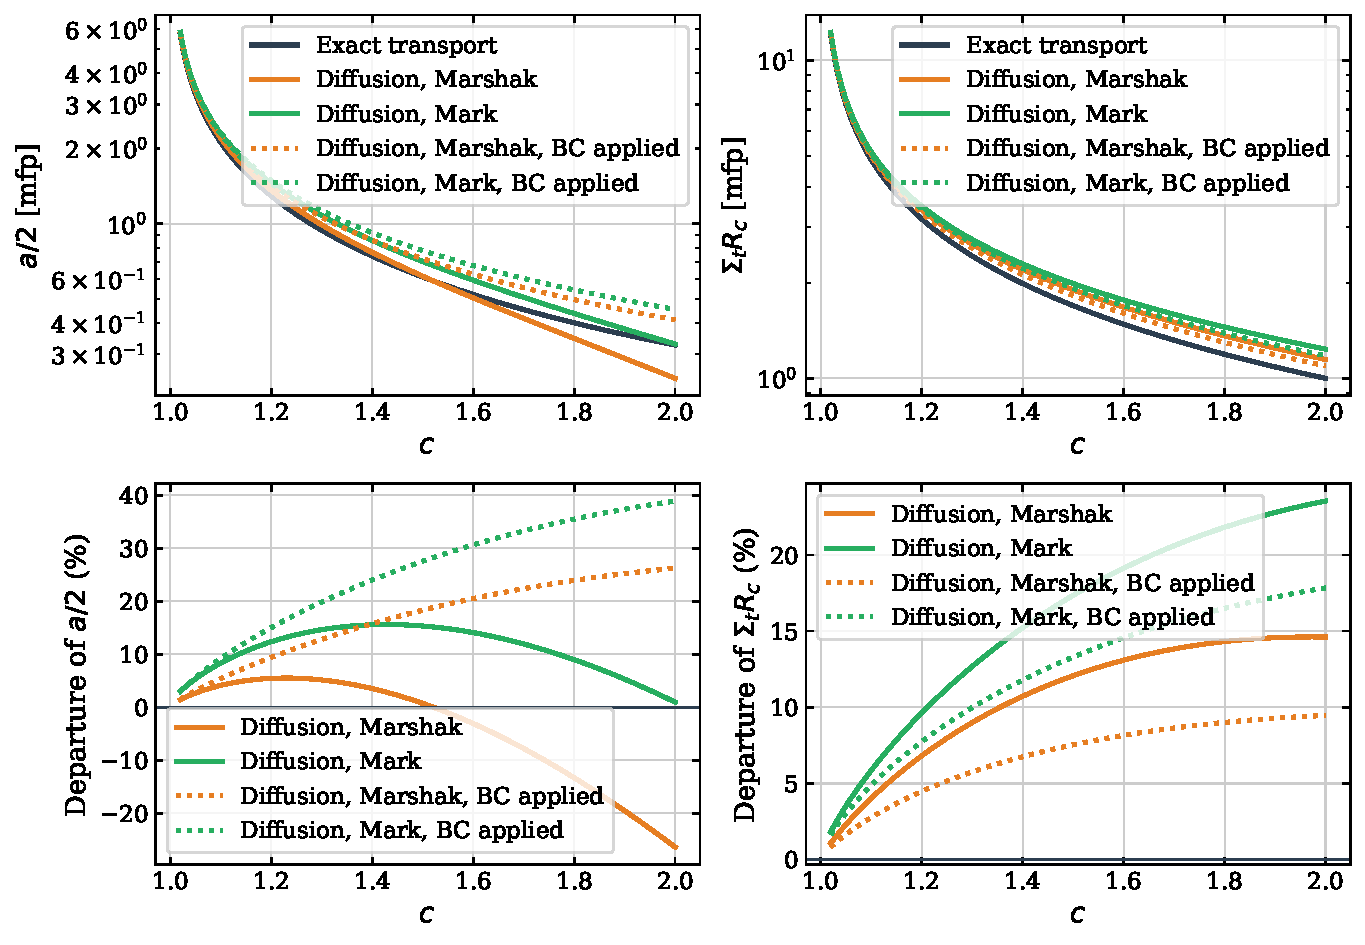
\includegraphics[width=\textwidth]{figs/q3_method_comparison.pdf}
    \caption{Exact transport against Marshak and Mark diffusion (top), and the signed departure of each from transport (bottom). Dotted curves impose the boundary condition on the flux shape instead of using an extrapolated zero.}
    \label{fig:q3_methods}
\end{figure}

\newpage
\FloatBarrier
\section*{Question 4: Numerical Diffusion Code in Spherical Coordinates}

The code solves
\begin{equation}
    -D \frac{1}{r^2} \frac{d}{dr}\left( r^2 \frac{d\phi}{dr} \right) + \Sigma_a \phi(r) = \frac{1}{k} \nu \Sigma_f \phi(r)
    \label{eq:q4_sphere}
\end{equation}
and finds the radius at which $k = 1$. Dividing the fission source by $k$ makes a solution exist at every radius, so criticality is a root search on $R$ rather than an eigenvalue search. Both approximations use the same solver, differing in two constants:
\begin{equation}
    \text{classical:} \quad D = \frac{1}{3\Sigma_t}, \quad z_0 = 2D,
    \qquad
    \text{asymptotic:} \quad D = \frac{(c-1)|\nu_0(c)|^2}{\Sigma_t}, \quad z_0 = z_0(c)
\end{equation}
The asymptotic $D$ is the continuation of Question 2's $(1-c)\nu_0^2$ above $c = 1$: both $\nu_0^2$ and $1-c$ change sign, so $D$ stays positive. Its purpose is to give the diffusion equation the true transport relaxation length $|\nu_0|/\Sigma_t$ instead of $1/\sqrt{3(c-1)}$.

\subsection*{Discretisation}

Finite volume on $N$ uniform cell-centred shells. Integrating \eqref{eq:q4_sphere} over cell $j$ turns the divergence into a difference of surface currents,
\begin{equation}
    A_{j+1/2} J_{j+1/2} - A_{j-1/2} J_{j-1/2} + \Sigma_a V_j \phi_j = S_j V_j,
    \qquad J_{j+1/2} = -D\,\frac{\phi_{j+1} - \phi_j}{h}
    \label{eq:q4_fv}
\end{equation}
with $A_i = 4\pi r_i^2$ and $V_j = \frac{4\pi}{3}(r_{j+1/2}^3 - r_{j-1/2}^3)$. The matrix is tridiagonal and solved in $O(N)$. Appendix~\ref{app:fv} works the mesh, the index map and the assembly through in full.

The outer boundary is the extrapolated zero: the mesh is run out to $R + z_0$ and the flux driven to zero there, which is what the Question 3 relations assume, so the comparison against them tests the numerics alone. Eliminating the surface flux between $\phi(R + z_0) = 0$ and the half cell separating it from the last centre gives the leakage coefficient
\begin{equation}
    J_s = \frac{D\,\phi_{N-1}}{h/2}
\end{equation}

\subsection*{The Iterative Algorithm}

$k$ comes from the source iteration of Bell \& Glasstone, pp.~189--192: start from a flat flux and $k = 1$. Form $S = \frac{1}{k}\nu\Sigma_f\phi$. Solve the removal problem $(-D\nabla^2 + \Sigma_a)\phi^{(n+1)} = S$. Update
\begin{equation}
    k^{(n+1)} = k^{(n)} \, \frac{\int \nu \Sigma_f \phi^{(n+1)} \, dV}{\int \nu \Sigma_f \phi^{(n)} \, dV}
\end{equation}
and repeat until $|k^{(n+1)} - k^{(n)}| < 10^{-10} k^{(n+1)}$. The flux is renormalised each sweep: its amplitude grows by roughly $k$ per sweep, and over several hundred sweeps the convergence test would otherwise lose its significant digits (This is physically irrelevant, since the ratio is homogeneous in $\phi$)

Convergence is at the dominance ratio $k_1/k_0$, which tends to unity for a large weakly multiplying sphere ($\approx 0.94$ at $c = 1.02$) and is derived under \emph{Verification} below. The critical radius then follows from Brent bisection on $k(R) - 1$, bracketed within $\pm 5\%$ of the analytic radius so that $k$ is never evaluated far from criticality.

\subsection*{Comparison with the Analytical Result}

At $k = 1$ equation \eqref{eq:q4_sphere} is Helmholtz with $B^2 = (\nu\Sigma_f - \Sigma_a)/D = \Sigma_t(c-1)/D$, and its regular solution $\sin(Br)/r$ vanishes at the extrapolated radius when
\begin{equation}
    R_c = \frac{\pi}{B} - z_0
    \label{eq:q4_analytic}
\end{equation}
Substituting the two parameter sets recovers the Question 3 relations exactly: $\Sigma_t R_c = \pi/\sqrt{3(c-1)} - 2/3$ classically, and $\Sigma_t R_c = \pi|\nu_0| - z_0(c)$ asymptotically, the latter being part 3(a). Note that $R_c$ depends on the cross sections only through $c$, since $\Sigma_a$ and $\nu\Sigma_f$ enter only as their difference.

\begin{table}[htbp]
    \centering
    \caption{Critical radius in mean free paths from the $k = 1$ search ($N = 400$) against \eqref{eq:q4_analytic}.}
    \label{tab:q4}
    \begin{tabular}{lccccc}
        \toprule
        & \multicolumn{2}{c}{Classical} & \multicolumn{2}{c}{Asymptotic} & \\
        \cmidrule(lr){2-3} \cmidrule(lr){4-5}
        $c$ & numerical & analytic & numerical & analytic & difference (classical) \\
        \midrule
        1.02 & 12.15881 & 12.15883 & 12.02752 & 12.02754 & $-1.6\times10^{-4}\,\%$ \\
        1.10 & 5.06906  & 5.06907  & 4.87295  & 4.87295  & $-1.7\times10^{-4}\,\%$ \\
        1.20 & 3.38911  & 3.38911  & 3.17289  & 3.17289  & $-1.8\times10^{-4}\,\%$ \\
        1.50 & 1.89843  & 1.89843  & 1.69369  & 1.69369  & $-2.1\times10^{-4}\,\%$ \\
        1.80 & 1.36122  & 1.36122  & 1.18995  & 1.18996  & $-2.3\times10^{-4}\,\%$ \\
        2.00 & 1.14713  & 1.14713  & 0.99952  & 0.99952  & $-2.4\times10^{-4}\,\%$ \\
        \bottomrule
    \end{tabular}
\end{table}

\subsection*{Verification}

Two further checks, independent of the comparison in Table~\ref{tab:q4}.

\paragraph{Convergence rate of the iteration.} The error of source iteration falls by the dominance ratio $k_1/k_0$ per sweep. With the spherical modes $B_n = n\pi/r_{\text{out}}$ this is $(\Sigma_a + DB_1^2)/(\Sigma_a + DB_2^2)$, which at a \emph{critical} radius collapses. Criticality means $\Sigma_a + DB_1^2 = \nu\Sigma_f$, and $B_2 = 2B_1$, so
\begin{equation}
    \frac{k_1}{k_0} = \frac{\nu\Sigma_f}{4\nu\Sigma_f - 3\Sigma_a} = \frac{c}{4c-3}
    \label{eq:dominance}
\end{equation}
The diffusion coefficient has cancelled: \emph{the convergence rate at criticality depends on $c$ alone}. 

\begin{table}[htbp]
    \centering
    \caption{Dominance ratio and sweep count to $|\Delta k| < 10^{-10}k$ at the critical radius. The sweep counts are identical for the classical and asymptotic approximations, as \eqref{eq:dominance} requires.}
    \label{tab:q4_iteration}
    \begin{tabular}{lccc}
        \toprule
        $c$ & $c/(4c-3)$ & sweeps \\
        \midrule
        1.02 & 0.944444 & 280 \\
        1.05 & 0.875000 & 133 \\
        1.10 & 0.785714 & \phantom{0}79 \\
        1.20 & 0.666667 & \phantom{0}50 \\
        1.50 & 0.500000 & \phantom{0}32 \\
        2.00 & 0.400000 & \phantom{0}25 \\
        \bottomrule
    \end{tabular}
\end{table}

\begin{figure}[htbp]
    \centering
    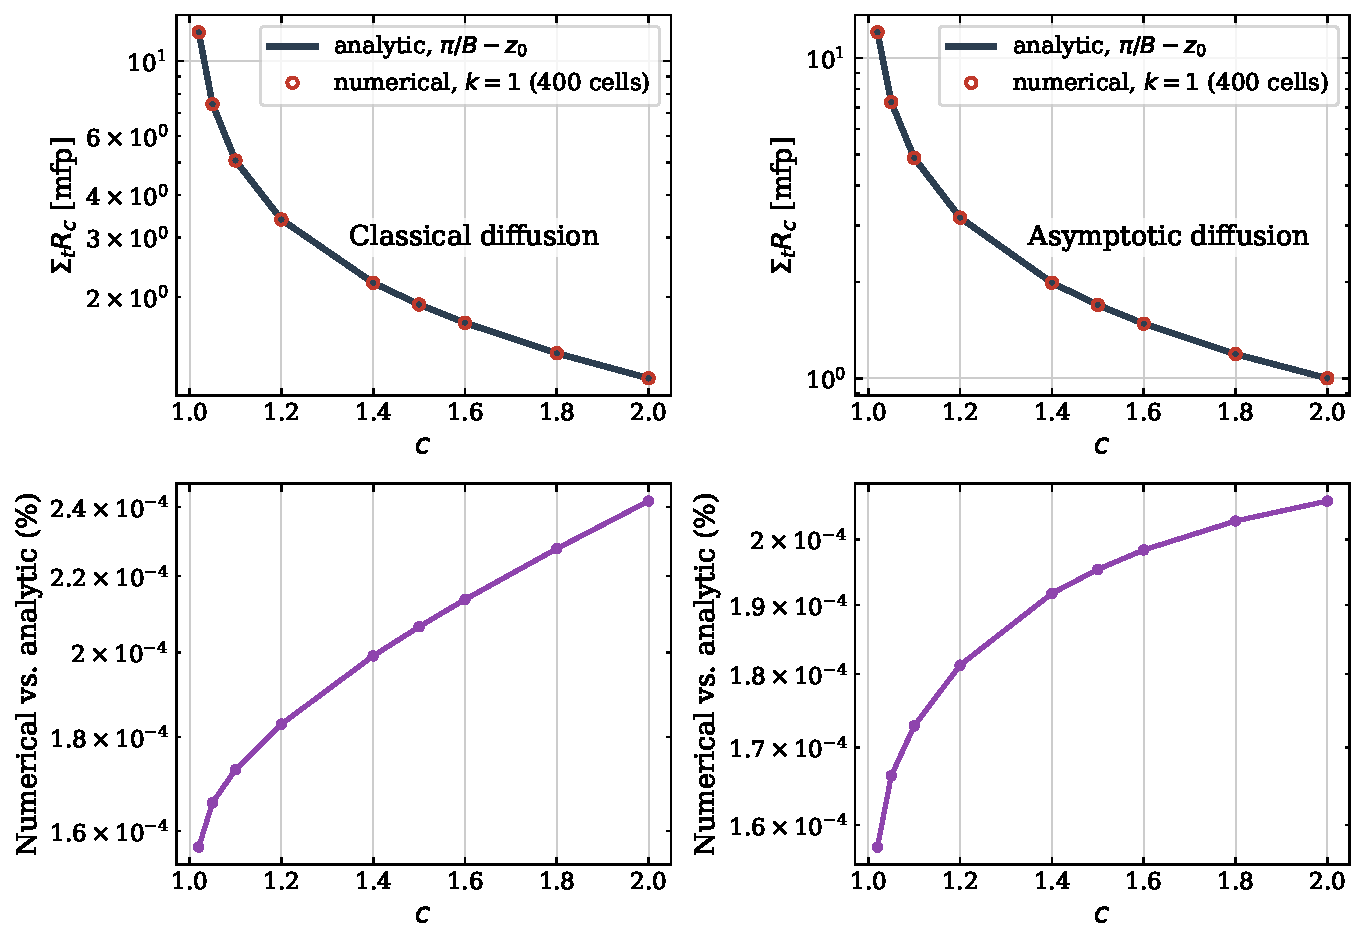
\includegraphics[width=\textwidth]{figs/q4_critical_radius.pdf}
    \caption{Critical radius from the $k = 1$ search (markers) against $\pi/B - z_0$ (solid), with the relative difference below.}
    \label{fig:q4_radius}
\end{figure}

\begin{figure}[htbp]
    \centering
    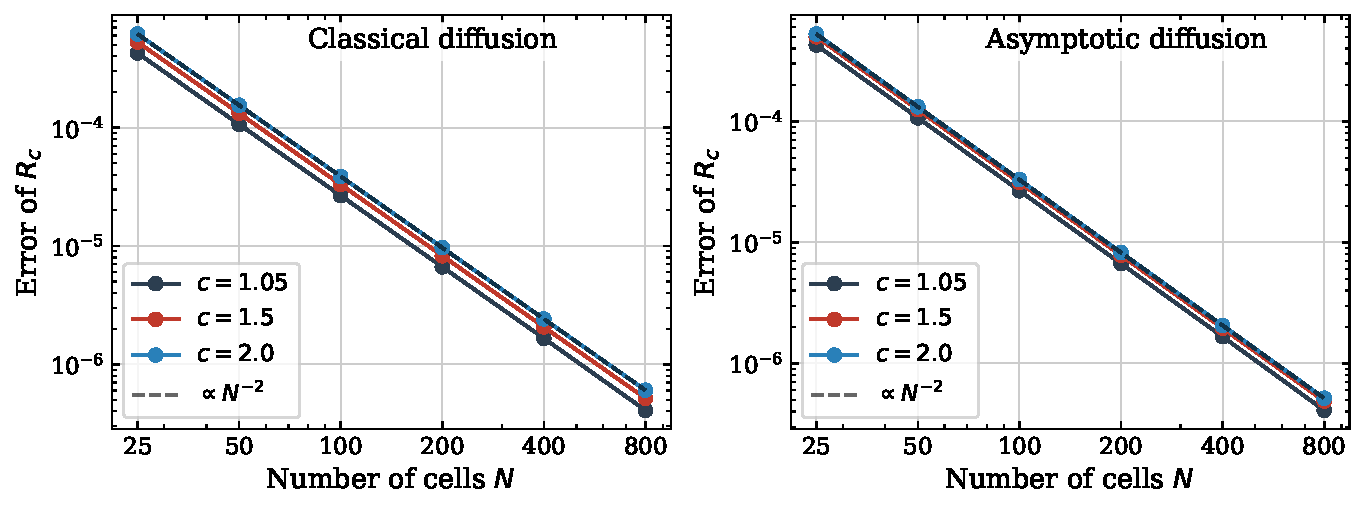
\includegraphics[width=\textwidth]{figs/q4_mesh_convergence.pdf}
    \caption{Mesh convergence of the critical radius, following the second-order guide $\propto N^{-2}$ at every refinement.}
    \label{fig:q4_convergence}
\end{figure}

\begin{figure}[htbp]
    \centering
    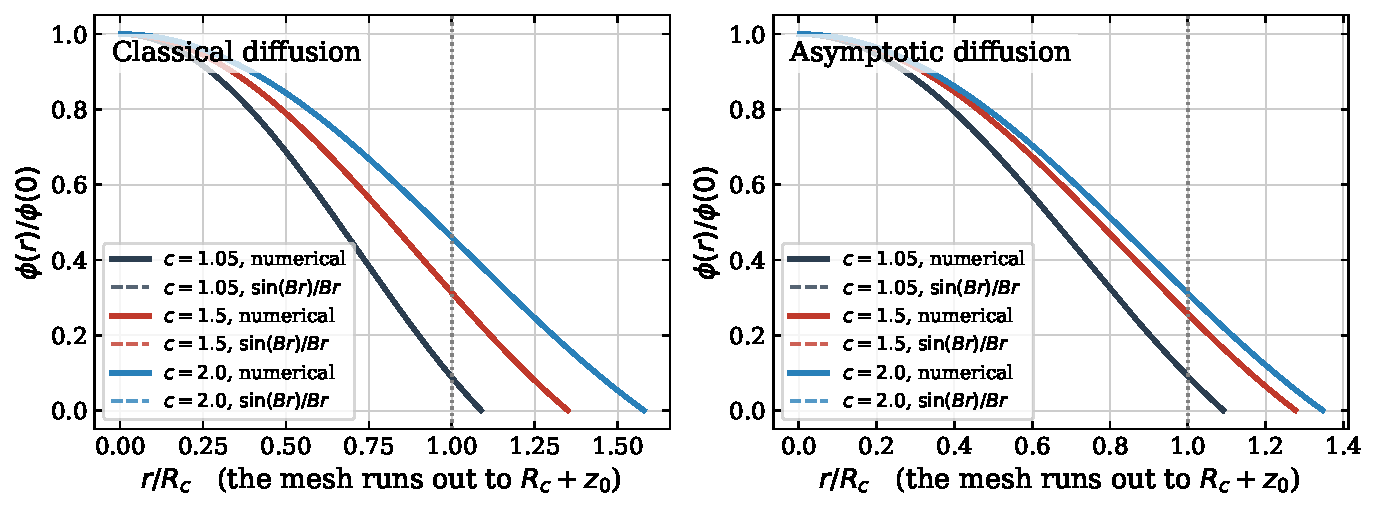
\includegraphics[width=\textwidth]{figs/q4_flux_profiles.pdf}
    \caption{Converged critical flux (solid) against the fundamental mode $\sin(Br)/Br$ (dashed), normalised at the centre. The mesh continues past $r/R_c = 1$ to the extrapolated radius, where the flux is driven to zero.}
    \label{fig:q4_flux}
\end{figure}

}

% The whole of Question 5 is one heading, one paragraph and two floats, so it is started on
% a fresh page and the table is barriered onto it: otherwise Question 4's backlog of floats
% lands between them and the section arrives as a mix of leftover figures and tables.
\clearpage
\section*{Question 5: Bare Critical Mass of U-235 and Pu-239}
Question 5 is Question 4 with the one-group benchmark cross sections of Sood, Forster \& Parsons (2003), the mass following as $M_c = \rho \frac{4}{3}\pi R_c^3$. Both fissile materials have $\Sigma_t = 0.32640$ cm$^{-1}$, a mean free path of $3.0637$ cm, so both critical spheres are about two mean free paths in radius.

\begin{table}[!ht]
    \centering
    \caption{Bare critical radius and mass from the $k = 1$ search on a 400-cell mesh. Numerical and analytic radii agree to four decimals in cm.}
    \label{tab:q5}
    \begin{tabular}{llccccc}
        \toprule
        Material & Approximation & $c$ & $\rho$ [g/cm$^3$] & $R_c$ [cm] & $\Sigma_t R_c$ & $M_c$ [kg] \\
        \midrule
        Pu-239 & classical  & 1.50 & 15.7 & 5.8163 & 1.8984 & 12.940 \\
        Pu-239 & asymptotic & 1.50 & 15.7 & 5.1890 & 1.6937 & \phantom{0}9.188 \\
        \midrule
        U-235  & classical  & 1.30 & 19.0 & 8.1031 & 2.6449 & 42.345 \\
        U-235  & asymptotic & 1.30 & 19.0 & 7.4339 & 2.4264 & 32.696 \\
        \bottomrule
    \end{tabular}
\end{table}
\FloatBarrier

\begin{figure}[htbp]
    \centering
    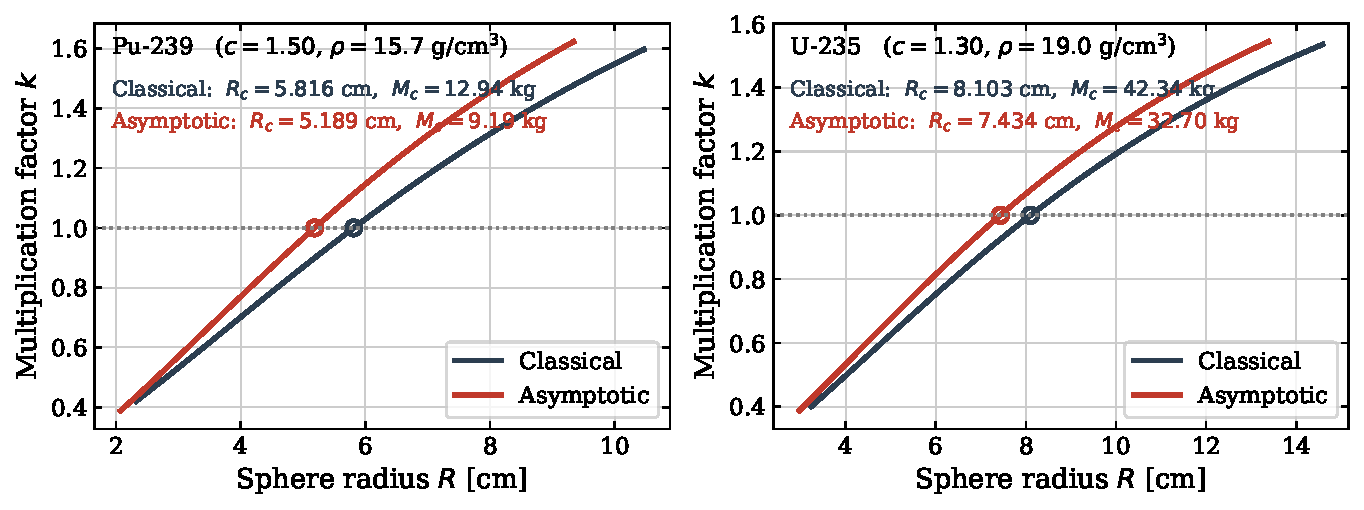
\includegraphics[width=\textwidth]{figs/q5_criticality.pdf}
    \caption{Multiplication factor against sphere radius for the two fissile materials, both approximations. The circles mark the $k = 1$ crossing.}
    \label{fig:q5}
\end{figure}

}

\clearpage
\appendix

{\color{red}

\section*{Appendix: The Spherical Finite-Volume Scheme in Detail}
\label{app:fv}

An expansion of Question 4's \emph{Discretisation}, following \texttt{src/homework1/spherical.py} line by line: what the mesh looks like, how \texttt{\_banded\_operator} turns it into a matrix, which index means what, and where the boundary conditions and the starting iterate enter.

\subsection*{The mesh and its indices}

\texttt{\_mesh} builds $N$ uniform cells on $[0, R_{\text{out}}]$ with $h = R_{\text{out}}/N$. Two families of index run over it and they must not be confused:

\begin{itemize}
    \item \textbf{Faces}, indexed $i = 0,\dots,N$ - there are $N+1$ of them, at radius $r_i = i h$, carrying areas $A_i = 4\pi r_i^2$ (\texttt{areas}, length $N+1$).
    \item \textbf{Cells}, indexed $j = 0,\dots,N-1$ - there are $N$ of them, cell $j$ spanning $[r_j, r_{j+1}]$, with centre $\bar r_j = (j + \tfrac12)h$ (\texttt{centres}) and volume $V_j = \tfrac{4\pi}{3}(r_{j+1}^3 - r_j^3)$ (\texttt{volumes}), both of length $N$.
\end{itemize}

Cell $j$ is bounded by face $i = j$ on the inside and face $i = j+1$ on the outside, so the two numberings share their integers. The rule that removes every ambiguity below is: \textbf{a subscript on $A$, $J$ or $C$ is a face. A subscript on $\phi$, $V$ or $S$ is a cell.} Where a relation ties a face to the two cells it separates, the same integer does double duty by construction - face $i$ has cell $i-1$ immediately inside it and cell $i$ immediately outside. The unknown $\phi_j$ is the average flux over cell $j$. It lives at the centre, not at a face. In the half-index notation of Question 4's \emph{Discretisation}, faces $i = j$ and $i = j+1$ are what were written $j - \tfrac12$ and $j + \tfrac12$. The integer form is used here because it is what the code indexes.

\begin{figure}[htbp]
\centering
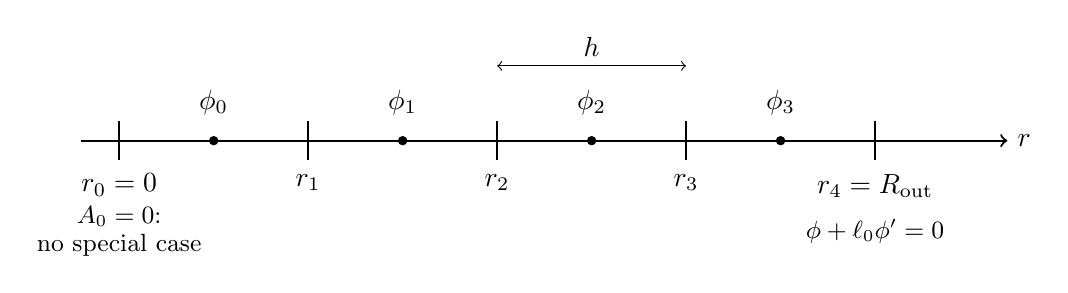
\begin{tikzpicture}[x=2.4cm, y=1cm]
    \draw[thick,->] (-0.2,0) -- (4.7,0) node[right] {$r$};
    \foreach \k in {0,1,2,3,4} \draw[thick] (\k,-0.25) -- (\k,0.25);
    \foreach \k/\lab in {0/{$r_0 = 0$},1/{$r_1$},2/{$r_2$},3/{$r_3$},4/{$r_4 = R_{\text{out}}$}}
        \node[below] at (\k,-0.3) {\lab};
    \foreach \i in {0,1,2,3} \fill (\i+0.5,0) circle (1.7pt);
    \foreach \i/\lab in {0/{$\phi_0$},1/{$\phi_1$},2/{$\phi_2$},3/{$\phi_3$}}
        \node[above] at (\i+0.5,0.2) {\lab};
    \draw[<->] (2,0.95) -- (3,0.95) node[midway,above] {$h$};
    \node[align=center] at (0,-1.15) {\small $A_0 = 0$:\\[-2pt] \small no special case};
    \node[align=center] at (4,-1.15) {\small $\phi + \ell_0 \phi' = 0$};
    \node at (2.5,-0.02) {};
\end{tikzpicture}
\caption{The cell-centred mesh for $N = 4$. Faces (ticks) carry areas, cells (dots) carry the unknowns. No unknown sits on a boundary, so both ends are face conditions rather than equations of their own.}
\label{fig:mesh}
\end{figure}

\subsection*{From the cell balance to a matrix row}

Rather than assume the balance \eqref{eq:q4_fv}, derive it from \eqref{eq:q4_sphere}: multiply by the volume element $4\pi r^2\,dr$ and integrate across cell $j$, from face $r_j$ to face $r_{j+1}$. The leading term is the one that matters, and the $r^2$ of the volume element is exactly what cancels the $1/r^2$ of the operator:
\begin{equation}
\begin{aligned}
    \int_{r_j}^{r_{j+1}} \left[-D\,\frac{1}{r^2}\frac{d}{dr}\!\left(r^2 \frac{d\phi}{dr}\right)\right] 4\pi r^2\,dr
    &= -4\pi D \int_{r_j}^{r_{j+1}} \frac{d}{dr}\!\left(r^2 \frac{d\phi}{dr}\right) dr \\[2pt]
    &= -4\pi D \left[\, r^2 \frac{d\phi}{dr} \,\right]_{r_j}^{r_{j+1}}
     \;=\; A_{j+1} J_{j+1} - A_j J_j
\end{aligned}
\label{eq:fv_derivation}
\end{equation}
using $A = 4\pi r^2$ and $J = -D\,d\phi/dr$. The integral of a divergence has collapsed onto the two faces - the divergence theorem for a shell - which is why nothing is ever evaluated at $r = 0$, where the operator itself is singular.

The other two terms integrate to volume averages by definition of the unknown, $\phi_j \equiv V_j^{-1}\!\int_{\text{cell } j} \phi \, dV$:
\begin{equation}
    \int_{r_j}^{r_{j+1}} \Sigma_a \phi \, 4\pi r^2 dr = \Sigma_a V_j \phi_j,
    \qquad
    \int_{r_j}^{r_{j+1}} \frac{\nu\Sigma_f \phi}{k} \, 4\pi r^2 dr = S_j V_j,
    \qquad S_j \equiv \frac{\nu\Sigma_f \phi_j}{k}
\end{equation}
Collecting the three gives \eqref{eq:q4_fv}, with the half-indices written as the integer face labels of \S\ref{app:fv}:
\begin{equation}
    A_{j+1} J_{j+1} - A_j J_j + \Sigma_a V_j \phi_j = S_j V_j
    \label{eq:fv_balance}
\end{equation}
Nothing has been approximated yet: this is an exact statement about cell averages and true face currents, for any $N$. \textbf{The discretisation enters only in the next step}, where the face current is replaced by a difference between neighbouring cell centres - which is also where the second-order accuracy under \emph{Verification} comes from. With Fick's law between adjacent centres, the current through face $i$ - which separates cells $i-1$ and $i$, a distance $h$ apart - is
\begin{equation}
    J_i = -D\,\frac{\phi_i - \phi_{i-1}}{h}
    \qquad\Longrightarrow\qquad
    A_i J_i = -C_i\,(\phi_i - \phi_{i-1}), \qquad
    \boxed{\;C_i \equiv \frac{D A_i}{h}\;}
\end{equation}
The \emph{conductance} $C_i$ is a property of a face, not of a cell - this is the whole idea of the layout.

Getting from \eqref{eq:fv_balance} to the matrix row takes three small steps, and the index change happens in the first of them. Cell $j$ has two faces, so the face relation is evaluated twice: at the inner face $i = j$, whose neighbours are cells $j-1$ and $j$, and at the outer face $i = j+1$, whose neighbours are cells $j$ and $j+1$. That substitution is where a face index becomes a pair of cell indices:
\begin{equation}
    A_j J_j = -C_j\,(\phi_j - \phi_{j-1}),
    \qquad
    A_{j+1} J_{j+1} = -C_{j+1}\,(\phi_{j+1} - \phi_j)
\end{equation}
Putting both into \eqref{eq:fv_balance}, the inner face carrying the minus sign of the balance and so flipping its bracket,
\begin{equation}
    \underbrace{-C_{j+1}\,(\phi_{j+1} - \phi_j)}_{\text{out through face } j+1}
    \;+\; \underbrace{C_j\,(\phi_j - \phi_{j-1})}_{\text{$-$(in through face } j)}
    \;+\; \Sigma_a V_j \phi_j = S_j V_j
\end{equation}
Expanding the brackets and collecting the three unknowns $\phi_{j-1}$, $\phi_j$, $\phi_{j+1}$:
\begin{equation}
    -C_j\,\phi_{j-1}
    + \left(C_j + C_{j+1} + \Sigma_a V_j\right)\phi_j
    - C_{j+1}\,\phi_{j+1}
    = S_j V_j
    \label{eq:fv_row}
\end{equation}
So cell $j$ couples to each neighbour through the conductance of the face it \emph{shares} with that neighbour - $C_j$ to the left, $C_{j+1}$ to the right - and both of those same two conductances reappear on the diagonal, because every neutron leaving through a face also leaves the cell it came from.
Each face appears in exactly the two rows it separates, with the same magnitude and opposite sign. That single fact gives the matrix all three of its useful properties: it is tridiagonal, it is symmetric, and it conserves neutrons exactly (\S\ref{app:properties}).

\subsection*{The two ends, and why neither needs a branch}

\paragraph{The origin.} Face $0$ sits at $r = 0$, so $A_0 = 0$ and therefore $C_0 = 0$. The $\phi_{-1}$ term in \eqref{eq:fv_row} vanishes on its own for cell $j = 0$, and no current crosses the centre. The symmetry condition $\phi'(0) = 0$ is thus imposed \emph{exactly}, by geometry, with no code path of its own - the reason \texttt{\_banded\_operator} can index a plain array at $j = 0$.

\paragraph{The outer surface.} Face $N$ has no cell beyond it. It sits at $R + z_0$, where the flux is driven to zero. Deriving its coefficient for the general condition $\phi + \ell_0 \phi' = 0$ and specialising afterwards is worth the extra line, because it shows the extrapolated zero is the clean $\ell_0 \to 0$ limit rather than a separate case. The surface flux $\phi_s$ is eliminated between that condition and the one-sided difference over the half cell $h/2$ that separates $\bar r_{N-1}$ from the surface:
\begin{equation}
    J_s = -D\phi'(R_{\text{out}}) = \frac{D\phi_s}{\ell_0},
    \qquad
    J_s = -D\,\frac{\phi_s - \phi_{N-1}}{h/2}
\end{equation}
Equating and solving,
\begin{equation}
    \phi_s = \phi_{N-1}\,\frac{\ell_0}{\ell_0 + h/2}
    \qquad\Longrightarrow\qquad
    J_s = \frac{D\,\phi_{N-1}}{\ell_0 + h/2},
    \qquad
    C_N = \frac{D A_N}{\ell_0 + h/2}
    \label{eq:CN}
\end{equation}
Because $\ell_0$ appears only in the denominator, $\ell_0 = 0$ is not a special case: it gives $\phi_s = 0$ and $C_N = D A_N/(h/2)$, which is the line \texttt{conductance[-1] = D * areas[-1] / (0.5 * h)} in \texttt{\_banded\_operator} and the only outer condition the code implements. The extrapolation distance has already been spent in placing the mesh boundary at $R_{\text{out}} = R + z_0$, so it does not appear again here.

Note where $C_N$ ends up: on the \emph{diagonal} of the last row only. It removes neutrons from cell $N-1$ without coupling it to anything, which is exactly what leakage out of the system is.

\subsection*{The banded storage, index by index}

Both indices of the matrix are cells: $M_{mn}$ couples cell $m$ to cell $n$. \texttt{scipy.linalg.solve\_banded((1, 1), ab, b)} expects it in diagonal-ordered form, meaning
\begin{equation}
    \texttt{ab}[\,1 + m - n,\; n\,] = M_{mn}, \qquad |m - n| \le 1
\end{equation}
so row $0$ of \texttt{ab} holds the superdiagonal, row $1$ the diagonal, row $2$ the subdiagonal - each stored in the \emph{column} of the entry, which is why the superdiagonal starts one slot in and the subdiagonal stops one slot early. The three assignments read:
\begin{center}
\begin{tabular}{ll}
    \toprule
    code & meaning \\
    \midrule
    \texttt{ab[0, 1:] = -conductance[1:-1]} & $M_{n-1,n} = -C_n$, \quad $n = 1..N{-}1$ \\
    \texttt{ab[1, :] = conductance[:-1] + conductance[1:]} & $M_{jj} = C_j + C_{j+1} + \Sigma_a V_j$ \\
    \phantom{\texttt{ab[1, :] = }}\texttt{+ sigma\_a * volumes} & \\
    \texttt{ab[2, :-1] = -conductance[1:-1]} & $M_{n+1,n} = -C_{n+1}$, \quad $n = 0..N{-}2$ \\
    \bottomrule
\end{tabular}
\end{center}
The face index survives in the conductance: the entry coupling cells $n-1$ and $n$ is $-C_n$, the conductance of face $i = n$, which is precisely the face they share.
The slices are the whole trick, and each says something physical:
\begin{itemize}
    \item \texttt{conductance[:-1]} is $C_0 \dots C_{N-1}$, the \emph{inner} face of each cell. \texttt{conductance[1:]} is $C_1 \dots C_N$, the \emph{outer} face of each cell. Element $j$ of their sum is the pair of faces bounding cell $j$ - the diagonal.
    \item \texttt{conductance[1:-1]} is $C_1 \dots C_{N-1}$, the $N-1$ \emph{interior} faces, i.e.\ precisely those that separate two cells. It is dropped into both off-diagonals unchanged, which is why $M$ comes out symmetric.
    \item The two excluded entries are the two boundaries: $C_0 = 0$ (nothing to couple across the origin) and $C_N$ (leakage, coupling to nothing).
\end{itemize}
For $N = 4$, with $C_0 = 0$ already substituted,
\begin{equation}
    M =
    \begin{pmatrix}
        C_1 + \Sigma_a V_0 & -C_1 & 0 & 0 \\
        -C_1 & C_1 + C_2 + \Sigma_a V_1 & -C_2 & 0 \\
        0 & -C_2 & C_2 + C_3 + \Sigma_a V_2 & -C_3 \\
        0 & 0 & -C_3 & C_3 + C_4 + \Sigma_a V_3
    \end{pmatrix}
\end{equation}
is stored as
\begin{equation}
    \texttt{ab} =
    \begin{pmatrix}
        \ast & -C_1 & -C_2 & -C_3 \\
        C_1 + \Sigma_a V_0 & C_1 + C_2 + \Sigma_a V_1 & C_2 + C_3 + \Sigma_a V_2 & C_3 + C_4 + \Sigma_a V_3 \\
        -C_1 & -C_2 & -C_3 & \ast
    \end{pmatrix}
\end{equation}
the two $\ast$ entries being the unused corners, left as the zeros \texttt{np.zeros} put there.

\subsection*{Two properties to check the assembly against}
\label{app:properties}

\paragraph{Symmetry and definiteness.} $M = M^{\!\top}$ because both off-diagonals are the same array, and the diagonal dominates strictly once $\Sigma_a > 0$ or $C_N > 0$. So $M$ is positive definite, the LU factorisation inside \texttt{solve\_banded} needs no pivoting, and the solve is $O(N)$.

\paragraph{Row sums are the neutron balance.} Summing row $j$ of \eqref{eq:fv_row}, the conductances cancel in pairs and leave $\Sigma_a V_j$ for every interior row - and $\Sigma_a V_{N-1} + C_N$ for the last. In matrix form,
\begin{equation}
    M \mathbf{1} = \Sigma_a \mathbf{V} + C_N \mathbf{e}_{N-1}
\end{equation}
that is: applied to a flat flux, the operator returns absorption plus surface leakage and nothing else. This is the discrete identity behind the balance check under \emph{Verification}. It holds by construction rather than by luck, which is why that check probes the boundary coefficient \eqref{eq:CN} and little else.

\subsection*{The source, $k$, and what plays the role of an initial condition}

Being a steady eigenvalue problem, this has no initial condition in the time-dependent sense. What it has instead is a \emph{starting iterate} for the power iteration, and it is worth being clear about which parts of the setup are physics and which are merely a starting guess:

\begin{itemize}
    \item \textbf{Baked into the matrix, once:} both boundary conditions. $C_0 = 0$ and $C_N$ are assembled before the first sweep, so every iterate - converged or not - satisfies them exactly. They are never re-imposed inside the loop.
    \item \textbf{The right-hand side} is the \emph{volume-integrated} fission source $F_j = \nu\Sigma_f \phi_j V_j$, divided by $k$. The factor $V_j$ is what makes it dimensionally consistent with the $C_i$'s, which are integrated currents. Compare \eqref{eq:fv_row}: the source term is $S_j V_j$, not $S_j$.
    \item \textbf{The starting guess} is a flat flux $\phi^{(0)}_j = 1$ with $k^{(0)} = 1$. Power iteration converges to the fundamental mode from any start with a non-zero component along it, which a strictly positive vector certainly has, so the converged $k$ and shape do not depend on this choice - only the number of sweeps does.
    \item \textbf{The renormalisation} $\phi \leftarrow \phi/\max\phi$ after each sweep is likewise not physics: the eigenvector is defined only up to scale, and both integrals in the $k$ update are homogeneous in $\phi$, so the factor cancels. It is there to keep the iterate at $O(1)$ so that the convergence test does not lose its significant digits.
\end{itemize}

The one quantity that does carry a physical scale through the whole calculation is the radius $R$: it fixes $R_{\text{out}}$, hence $h$, hence every area, volume and conductance. That is the sense in which the outer root search of \texttt{critical\_radius} sits outside everything described here - each evaluation of $k(R)$ rebuilds the mesh and the matrix from scratch.

}

\end{document}
